\input{preamble_ida14}
\raggedbottom
\begin{document}

\include{filer/Underskrifter}

% Resume

% Resume

\chapter*{Resume}
Følgende rapport og tilhørende dokumentation beskriver arbejdet med gruppens semesterprojekt for 3. semester på Aarhus School of Engineering. Formålet med projektet er at afprøve de metoder og emner som semesterets fag har introduceret. Rapporten beskriver arbejdsmetoderne der er brugt fra idé til produkt, det egentlige produkt og udviklingen af dette samt de overvejelser og værktøjer som er benyttet. Dokumentationen indeholder en udtømmende teknisk beskrivelse af systemet.

Udgangspunktet for systemet er at kunne styre vanding af goldbaner på en nem og simpel måde. Fra et computerprogram kan en bruger styre systemets dele og fastlægge grænser for hvornår vanding skal starte mv. Autonome enheder placeres rundt på goldbanens huller og fra disse enheder distribueres et netværk af sensorer som overvåger de miljømæssige data.

Udviklingsforløbet er styret efter ASE-modellen, som er en halv-iterativ projektledelsesmetode. Produket er udviklet på to forskellige platforme. Brugerinteraktion sker igennem Devkit8000-platformen og det autonome system anvender PSoC4-boardet fra Cypress samt egen udviklet hardware til sensor-håndteringen. 

Projektet er endt ud i et funktionelt system som kan aflæse data fra sensorerne og reagerer på disse. Selve vand-pumpe-konstruktionen til vanding af banerne er kun lavet som en simpel konceptuel opstilling.

% English Abstract

% Abstract
\chapter*{Abstract}

The following document describes the work and process of the groups 3rd term project at Aarhus School of Engineering. The purpose of the project is to use and evaluate the methods and subjects taught at this terms courses. The report describes how the product came from an idea to a physical product as well as the details of the product and the methods used. The documentation holds all technical details about the product.

The product developed is an automatic watering system that helps controlling the environment around gold courses. From a computer program the user can control the whole system and set the limits from which the autonomous system reacts. The autonomous units are placed along the fairways with a grid of sensors placed in the ground on the fairway collecting environmental data.

Development is managed with the ASE-model, which is a semi-iterative project management process. Further more is it done on two different platforms namely the Devkit8000 for the user interaction component and the PSoC4 from Cypress as the core of the autonomous system along with specialised hardware for the sensors.

The results include a functional user interface and a fully established data-collection system. Though limited by the implementation of the water pump system, which is suppressed due time restrictions.

\afterpage{\null\newpage} % Indholdsfortegnelse skal starte på højre side

% Indledning

\tableofcontents*

Gruppen vil udvikle et system til vanding af golfbaner. I forbindelse med stigende temperature bliver det mere kritisk at vandingen af golfbaner sker på de rigtige tidspunkter for at holde banen spilbar. For at spare på resourcerne er det også kritisk ikke at spilde store mængder vand på vanding af områder som ikke trænger til det.

Med et system af intelligente enheder der kan arbejde autonomt, men som modtager indstillinger for vandingen fra en masterenhed, herved kan man spare arbejdstid for greenkeeperen og vandingen sker kun når det er nødvendigt.

Normalt vil man placere en af disse enheder ved hvert hul på golfbanen og lave et netværk af sensorer lokalt til denne enhed. Den kan dermed overvåge området og vande om nødvendigt. Alle enhederne forbindes til et netværk som er koblet sammen med Master. Grænseværdierne, for f.eks. jordfugtigheden, der afgør hvornår enheden skal påbegynde vanding kommer fra Master og styres igennem denne af greenkeeperen. 

\begin{figure}[ht] \centering
\fbox{\includegraphics[height=4.1cm]{filer/indledning/billeder/hul_med_sprinkler}}
\caption{Systemoverblik}
\label{fig:systemoverblik}
\end{figure}

FIGURBESKRIVELSE MANGLER!!!

Oversigt over blokkene i systemet kan ses i figur \ref{fig:bloksystemoverblik}.
Bemærk at der er muligt at forbinde flere af hver type sensor til én enhed. Hvis altså et hul på en golfbane kræver tre temperatursensorer, kobles disse blot på den samme enhed.

\begin{figure}[ht] \centering
\fbox{\includegraphics[height=10cm]{filer/indledning/billeder/vandingssystem}}
\caption{Blokoverblik af system}
\label{fig:bloksystemoverblik}
\end{figure}

FIGUREN HEROVER SKAL DISKUTERES PÅ MØDE!

Systemet laves med en PSoC som Enhed, altså den del der håndterer data fra sensorene mv.
Devkit8000 fungerer som Master og er brugerinterface.

En Enhed består altså af:
\begin{enumerate}
\item Fugtighedssensor (evt. flere)
\item Temperatursensor (evt. flere)
\item Bevægelsessensor (evt. flere)
\item Sprinkler (evt. flere)
\item PSoC controller board
\end{enumerate}

Fugt- og temperatursensorerne registrerer banens behov for vanding. Bevægelsessensoren registrerer om der er spillere på det pågældende hul. Sprinkleren sørger for vandingen når der skal vandes. Denne skjules nede i græsset og kommer op når vandingen skal være aktiv.
PSoC controller-boardet bliver hjernen i Enheden. Denne styrer kommunikationen til Master og holder styr på de generelle funktioner for Enheden så som udlæsning af data, aktivering af sprinkler mv.

% Opgave formulering

\chapter{Opgaveformulering (MK PO)}

Konstruer et system til vanding af golfbaner. Systemet skal indeholde én Master (Devkit8000) som kontrollerer et netværk af Enheder (PSoC4). Kommunikationen mellem Master og Enhed skal foregå via den serielle kommunikation kaldet SPI. Via denne kommunikation skal Masteren kunne kontrollere de enkelte Enheder, samt indhente log-data fra disse. 
Enheden skal fungerer autonomt, når denne er aktiveret. Enheden  er tilkoblet en komponentpakker bestående af fugt- og temperatursensor samt sprinkler med tilhørende pumpe og vandforsyning. Enheden skal således selv styre vanding af trængende områder. En bevægelsessensor skal placeres ved indgangen til hvert golfhul, hvis der registreres bevægelse blokeres en evt. vanding i 30 minutter.  

Figur \ref{fig:systemoversigt} illustrerer ovenstående.  

%SYSTEMOVERBLIK BILLEDE
\begin{figure}[h]
  \centering
    \includegraphics[width=\textwidth]{Billeder/systemoversigt}
    \caption{Systemoversigt}
    \label{fig:systemoversigt}
\end{figure}


% Afgrænsniger i projektet

\chapter{Projektafgrænsning (JS)}
%afgrænsninger i projektet her.

Et fuldt integreret vandingssystem er, grundet manglende ressourcer og tid, ikke en mulighed på dette semesterprojekt, men der udarbejdes i stedet en skaleret prototype.
Foruden størrelsesbegrænsning er der fra skolens side givet forbud mod, uanset tidligere baggrund, at der arbejdes på 230V, men da der indgår en 230V pumpe i projektet har skolen givet særtilladelse til at der laves et relæ-kredsløb i en lukket kasse, hvori alle ledende dele er helt afskærmet for fysisk kontakt som kan ses på figur \ref{lab:230Vrelay}.

Hurtigt i projektets forløb fik vi tildelt en pumpe fra Grundfos, det viste sig senere at denne ikke kunne bruges til det ønskede formål med at skabe et vandtryk, da denne er en cirkulationspumpe. 

%Løsningen på dette ender med en billig vandpumpe til påmontering på en 230 V %boremaskine. 

\begin{figure}[H]
  \centering
    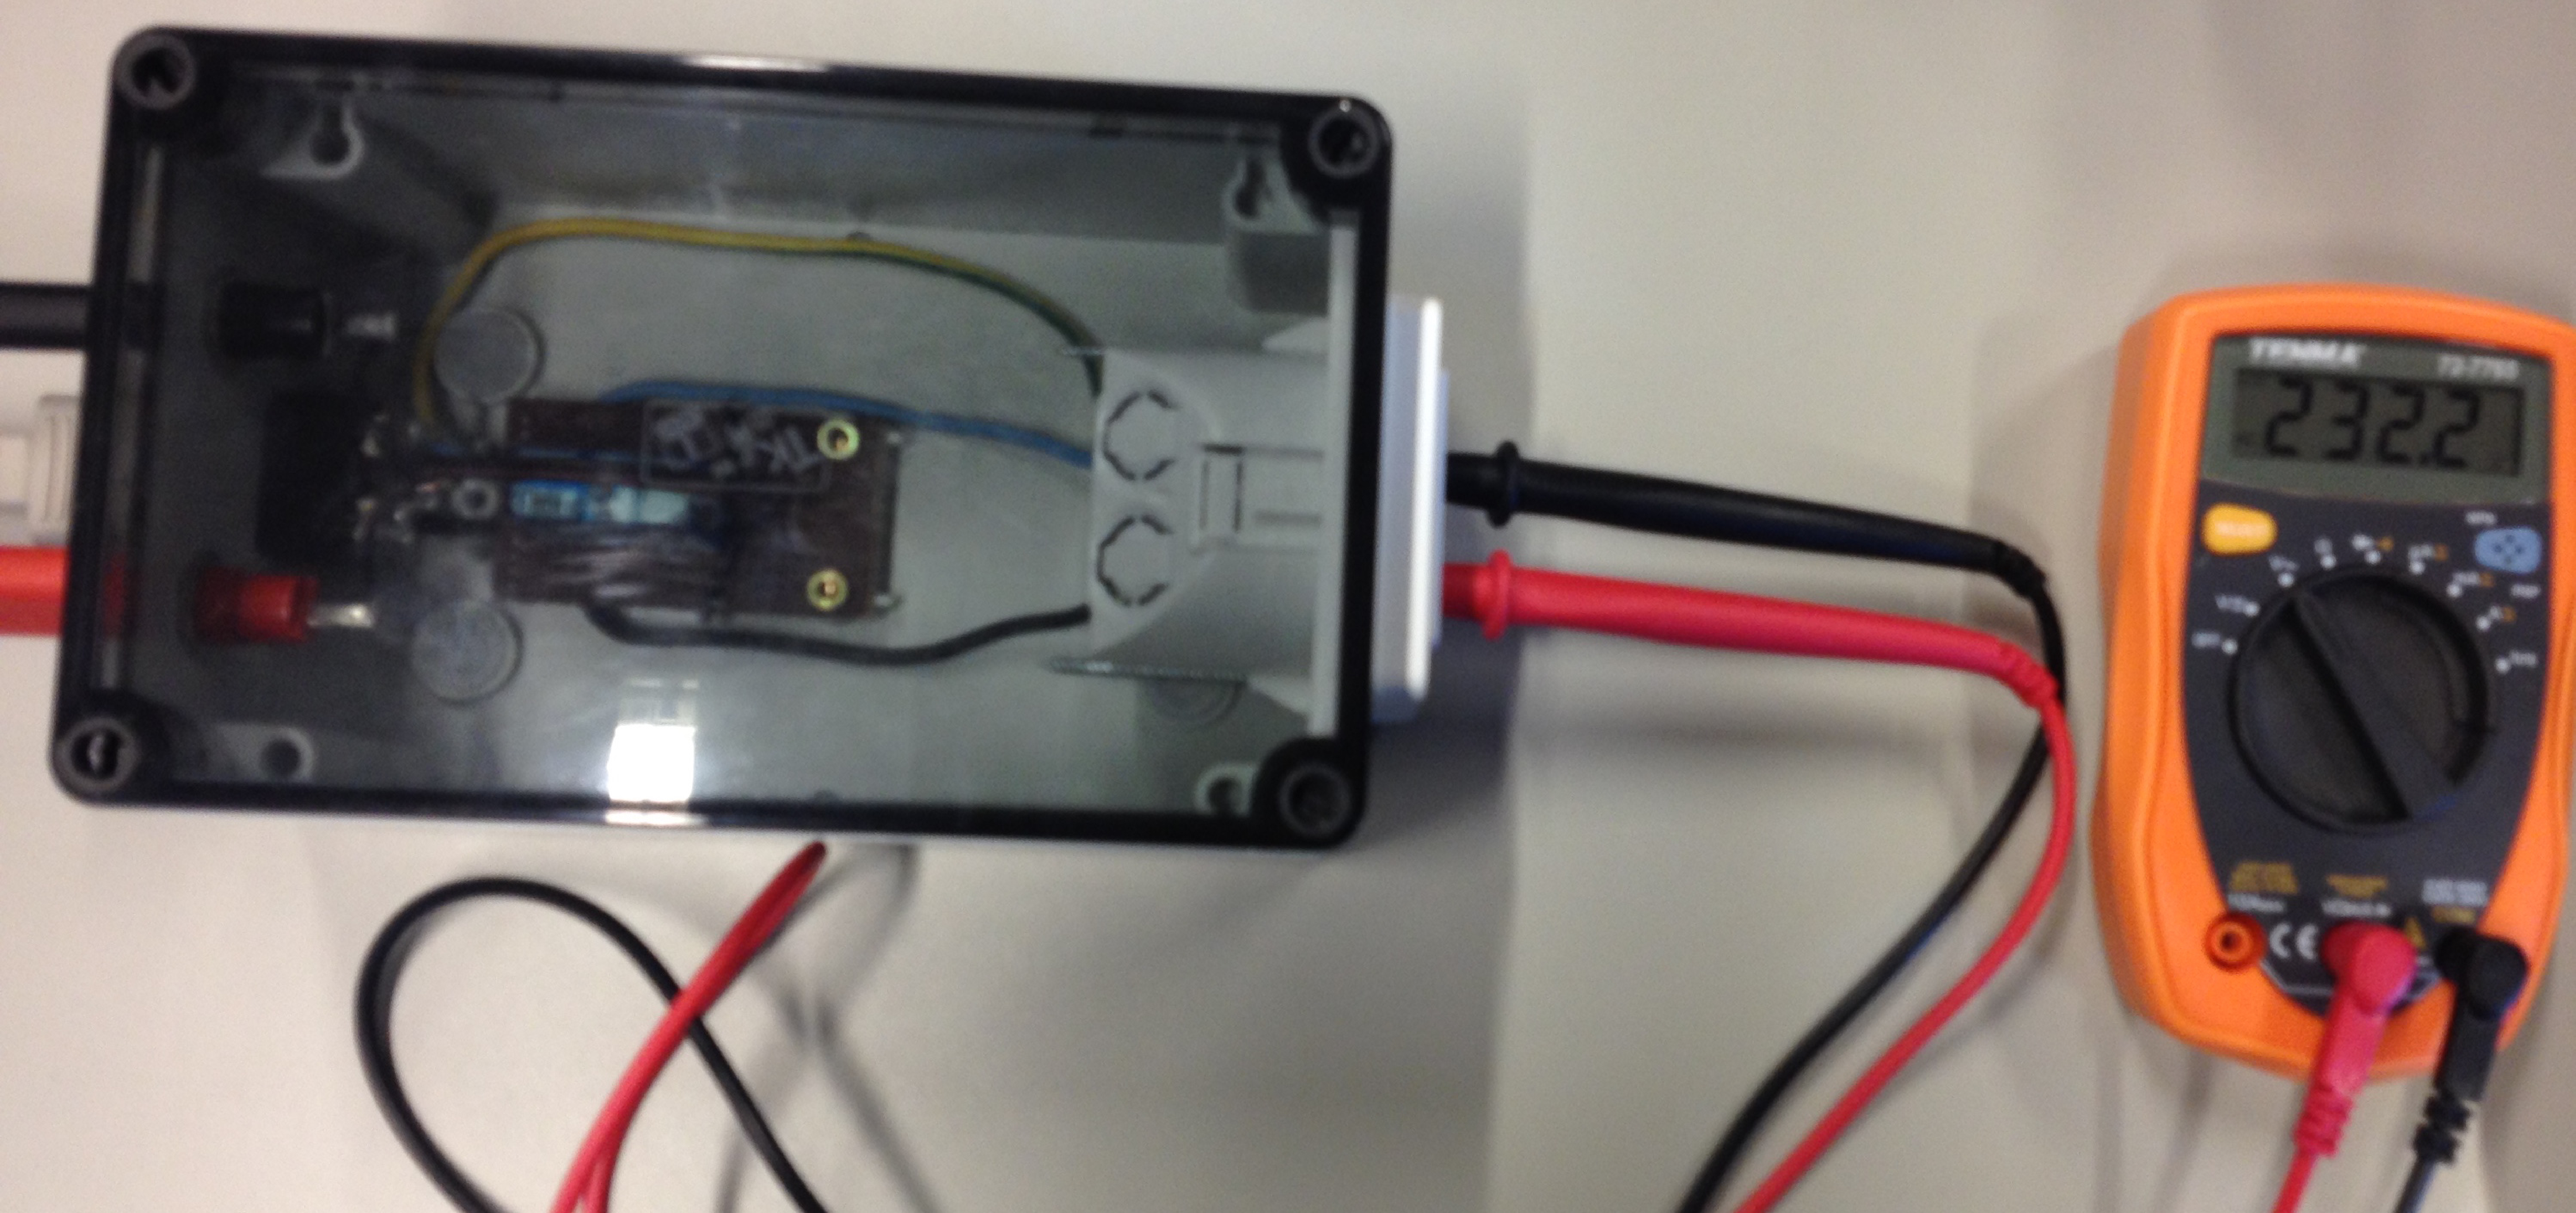
\includegraphics[width=0.75\textwidth]{Billeder/230Vrelay}
    \caption{Relæ i afskærmet kasse}
    \label{lab:230Vrelay}
\end{figure}

Efter at den serielle kommunikation(SPI) var implementeret færdig og klar til test, viste det sig at overførelsesafstanden på 22 cm, som først var tiltænkt, ikke kunne lade sig gøre, da dataen blev korrupt undervejs. Denne afstand blev da nedsat til 7 cm for at kunne overføre data uden fejl.
 



% Systembeskrivelse

\chapter{Systembeskrivelse (MK PO)}

EasyWater8000 er et samlet vandingssystem, hovedsagligt målrettet imod vanding af en golfbane. Her følger en detaljeret beskrivelse af systemet.

\begin{figure}[H]
  \centering
    \includegraphics[width=0.9\textwidth]{billeder/systembeskrivelse}
    \caption{Oversigt over det samlede system}
    \label{fig:systembeskrivelse}
\end{figure}

Figur \ref{fig:systembeskrivelse} viser et simplificeret overblik over hvad EasyWater8000 består af. Der er en Master, som er hovedcomputeren i systemet med Linux(Angstrom) som styresystem. Masteren kommunikerer og styrer op til 18 Enheder der hver har en komponentpakke og en bevægelsessensor tilsluttet.

Komponentpakken er en samling af 3 komponenter, en temperatursensor og en fugtsensor til at hhv. måle temperaturen og fugtigheden i jorden omkring komponentpakken, samt en sprinkler til at vande græsset og jorden i samme område.

Bevægelsessensoren sidder ved hvert teested på golfbanen, og registrerer bevægelse i det område. Når der bliver registreret bevægelse vil sensoren give signal til at deaktivere vandingen på det givne golfhul, så golfspillerne ikke bliver utilsigtet våde.

Et golfhul kunne se ud som på Figur \ref{fig:hul_med_sprinkler}

\begin{figure}[H]
  \centering
    \includegraphics[width=\textwidth]{billeder/hul_med_sprinkler}
    \caption{Eksempel på golfbane med sprinklere}
    \label{fig:hul_med_sprinkler}
\end{figure}

Enhederne kører autonomt, dvs. de selv monitorerer fugt og temperatur og vander hvis grænserne overskrides. Enhederne får deres grænseværdier fra Masteren og logger sine målte data til Masteren, via SPI transmission.

% Kravspec

\chapter{Krav}
EasyWater8000 er et system udviklet med henblik på at lette greenkeeperens opgave med at holde græsset på golfbanen. Systemet skal automatisk tænde for sprinklerne på golfbanen når den bliver for tør eller temperaturen bliver for høj. Dette gør at greenkeeperen ikke selv skal tænde for det eller sætte faste vandingstidspunkter, men at græsset bliver vandet når det har brug for det. Systemet måler både fugt og temperatur, al data samles i en log som kan printes på styringen (Masteren).  Desuden observerer systemet om en person eller spiller går ind på banen og deaktiverer vandingssystemet i en periode for systemet ikke vander hullet mens spilleren er derpå. 

Greenkeeperen kan fra styringen sætte en række værdier for hvor tørt og varmt der skal være før der vandes. Når værdierne er sat kan systemet køre af sig selv. Greenkeeperen kan også tvinge en vanding igennem hvis der f.eks. er en konkurrence næste dag og golfbanen således ikke vandes hele dage da der er personer derpå hele tiden. 

% generelle krav for systemet 

\chapter{Kravspecifikation}

\clearpage

% Indledning

\section{Indledning}
Gruppen vil udvikle et system til vanding af golfbaner. I forbindelse med stigende temperature bliver det mere kritisk at vandingen af golfbaner sker på de rigtige tidspunkter for at holde banen spilbar. For at spare på resourcerne er det også kritisk ikke at spilde store mængder vand på vanding af områder som ikke trænger til det.

Med et system af intelligente enheder der kan arbejde autonomt, men som modtager indstillinger for vandingen fra en masterenhed, herved kan man spare arbejdstid for greenkeeperen og vandingen sker kun når det er nødvendigt.

Normalt vil man placere en af disse enheder ved hvert hul på golfbanen og lave et netværk af sensorer lokalt til denne enhed. Den kan dermed overvåge området og vande om nødvendigt. Alle enhederne forbindes til et netværk som er koblet sammen med Master. Grænseværdierne, for f.eks. jordfugtigheden, der afgør hvornår enheden skal påbegynde vanding kommer fra Master og styres igennem denne af greenkeeperen. 

\begin{figure}[ht] \centering
\fbox{\includegraphics[height=4.1cm]{filer/indledning/billeder/hul_med_sprinkler}}
\caption{Systemoverblik}
\label{fig:systemoverblik}
\end{figure}

FIGURBESKRIVELSE MANGLER!!!

Oversigt over blokkene i systemet kan ses i figur \ref{fig:bloksystemoverblik}.
Bemærk at der er muligt at forbinde flere af hver type sensor til én enhed. Hvis altså et hul på en golfbane kræver tre temperatursensorer, kobles disse blot på den samme enhed.

\begin{figure}[ht] \centering
\fbox{\includegraphics[height=10cm]{filer/indledning/billeder/vandingssystem}}
\caption{Blokoverblik af system}
\label{fig:bloksystemoverblik}
\end{figure}

FIGUREN HEROVER SKAL DISKUTERES PÅ MØDE!

Systemet laves med en PSoC som Enhed, altså den del der håndterer data fra sensorene mv.
Devkit8000 fungerer som Master og er brugerinterface.

En Enhed består altså af:
\begin{enumerate}
\item Fugtighedssensor (evt. flere)
\item Temperatursensor (evt. flere)
\item Bevægelsessensor (evt. flere)
\item Sprinkler (evt. flere)
\item PSoC controller board
\end{enumerate}

Fugt- og temperatursensorerne registrerer banens behov for vanding. Bevægelsessensoren registrerer om der er spillere på det pågældende hul. Sprinkleren sørger for vandingen når der skal vandes. Denne skjules nede i græsset og kommer op når vandingen skal være aktiv.
PSoC controller-boardet bliver hjernen i Enheden. Denne styrer kommunikationen til Master og holder styr på de generelle funktioner for Enheden så som udlæsning af data, aktivering af sprinkler mv.

% Aktører

\section{Aktører}
Her beskrives systemets aktøre. Disse vil blive refereret i de efterfølgende usecase-beskrivelser.

%% !!! Aktør kontekst diagram !!!
%
%\fbox{\includegraphics[width=0.9\textwidth]{billeder/diagrammer/Kontekst_Diagram}}
%\caption{Kontekst diagram}
%\label{lab:kontekstdiagram}
%\end{figure}

\begin{table}[!htbp] \centering
	\begin{tabular}{|p{2.5cm}|p{11.5cm}|}
	\hline
		\textbf{Aktør navn} & \textbf{Beskrivelse} \\\hline
		Bruger & Bruger-aktøren vil normalt være greenkeeperen. Det er vedkommende som kontrollere og betjener systemet. (Primær) \\\hline

		Omgivelser & Almene omgivelser, som har indflydelse på systemets sensorer. Det være sig temperatur, fugtighed og bevægelser i områderne omkring systemet. (Sekundær) \\\hline
	\end{tabular}
\end{table}

Ud over de nævnte aktører bruges også navnene på nogle af systemets dele.


% Usecases

\section{Usecases}

Her følger en dybere beskrivelse af systemets opbygning og måde at virke på. Dette gøres med fulde usecase beskrivelser hvor systemets virkning er beskrevet i detaljer.

\begin{figure}[!htbp] \centering
\vspace*{\fill}
\includegraphics[width=\textwidth]{filer/kravspec/visio/Usecase_Diagram}
\caption{Usecase diagram}
\label{lab:usecasediagram}
\vspace*{\fill}
\end{figure}

%% !!! Use case diagram !!!
%
%\begin{figure}[!htbp] \centering
%\section{Usecases}
%\vspace*{\fill}
%\includegraphics[width=\textwidth]{billeder/diagrammer/Usecase_Diagram}
%\caption{Usecase diagram}
%\label{lab:usecasediagram}
%\vspace*{\fill}
%\end{figure}

% UC1: Indsamle data

\subsection{UC1: Tilføj/fjern enhed}
\begin{center} \centering \label{UC1}
	\begin{longtable}{|p{5cm}|p{9cm}|}  %% Longtable = forsætter på næste side
	\hline
		\multicolumn{2}{|l|}{\textbf{UC1: Tilføj\slash fjern enhed}} \\\hline %% HUSK UCECASE NUMMER + NAVN
		\endfirsthead
		
		\multicolumn{2}{l}{...fortsat fra forrige side} \\ \hline %% Til LONGTABLE
		\multicolumn{2}{|l|}{\textbf{UC1: Tilføj\slash fjern enhed}} \\\hline %% HUSK UCECASE NUMMER + NAVN
		\endhead	
		
		\textbf{Mål}								&Bruger kan tilføje eller fjerne enheder fra systemet			\\\hline
		\textbf{Initialisering}					&Bruger														\\\hline
		\textbf{Aktører og Stakeholders}			&Bruger(Primær)												\\\hline 
		\textbf{Referencer}						&Ingen														\\\hline
		\textbf{AASH}							&1															\\\hline
		\textbf{Efterfølgende tilstand}			&Ønsket Enhed er tilføjet eller fjernet fra systemet.		\\\hline
		\textbf{Hovedforløb}					
			&\begin{enumerate}
	
				\item Bruger vælger ''Tilføj/fjern enhed'' i hovedmenu
				
				\item \label{uc1valg} Bruger vælger ''Tilføj enhed''
				
				\item En liste af opsatte enheder præsenteres på skærmen				
				
				\begin{enumerate}
					\item \label{uc1indtast} Master beder bruger om at indtaste informationer
					
					\item \label{uc1indtast_fejl} Bruger indtaster \textcolor{red}{navn og adresse} på Enhed
					
						\textbf{[Undtagelse \ref{uc1indtast_fejl}.a]} \newline
						Indtastede værdier er ikke gyldige
					
					\item Master tilføjer Enhed til systemet med default parametre
					
					\item Enhed forbindes til kommunikationsnetværket
					
					\item \label{uc1verif} Master verificerer forbindelsen til Enhed og sender dato og tidspunkt
						
					\textbf{[Undtagelse \ref{uc1verif}.a]} \newline
					Enheden kan ikke verificeres
					
					\item Enhed gemmer dato og tidspunkt
				\end{enumerate}

				\item Bruger vælger ''Fjern enhed''

				\item En liste af opsatte enheder præsenteres på skærmen

				\begin{enumerate}
					
					\item Bruger indtaster adresse på Enhed
					
					\item Master deaktivere Enhed
					
					\item Master sletter Enhed fra systemet
				
				\end{enumerate}
				
				\item Master opdaterer liste med opsatte enheder
				
				\item Bruger kan returnere til hovedmenu eller opsætte ny enhed (Gå til UC1.\ref{uc1valg})
			\end{enumerate}\\\hline
		\textbf{Undtagelser}
			&\begin{enumerate}[label=\ref{uc1indtast}.a]
				
				\item Master viser fejlbesked omkring ugyldige værdier
				
					\subitem Gå til UC1.\ref{uc1indtast}
			\end{enumerate}
			
			\begin{enumerate}[label=\ref{uc1verif}.a]
				
				\item Master viser fejlbesked angående verificering af enheden
				
				\item Bruger kan forsøge igen (Gå til UC1.\ref{uc1verif} eller afbryde)

			\end{enumerate}														\\\hline
	\end{longtable} 
\end{center}

%% TIPS:
%% LABEL TIL PUNKT: \label{labelnavn}
%% REFERENCE: \ref{labelnavn}

% UC2: Aktiver/Deaktiver

\subsection{UC2: Config}
\begin{center} \centering \label{UC2}
	\begin{longtable}{|p{5cm}|p{9cm}|}  %% Longtable = forsætter på næste side
	\hline
		\multicolumn{2}{|l|}{\textbf{UC2: Konfig}} \\\hline %% HUSK UCECASE NUMMER + NAVN
		\endfirsthead
		
		\multicolumn{2}{l}{...fortsat fra forrige side} \\ \hline %% Til LONGTABLE
		\multicolumn{2}{|l|}{\textbf{UC2: Konfig}} \\\hline %% HUSK UCECASE NUMMER + NAVN
		\endhead	
		
		\textbf{Mål}								&Ændre default parametre på en Enhed			\\\hline
		\textbf{Initialisering}					&Bruger							\\\hline
		\textbf{Aktører og Stakeholders}			&Bruger(Primær)					\\\hline
		\textbf{Referencer}						&Ingen							\\\hline
		\textbf{AASH}							&1								\\\hline
		\textbf{Efterfølgende tilstand}			&Ingen							\\\hline
		\textbf{Hovedforløb}					
			&\begin{enumerate}
	
				\item Bruger vælger ''Konfig'' i hovedmenu
				
				\item \label{uc2afbryd}Bruger vælger den Enhed, der ønskes omkonfigureret.\newline
				\textbf{[Undtagelse \ref{uc2afbryd}.a]} \newline
					Bruger vælger afbryd
				
				\item \label{uc2afbryd2}Bruger ændrer parametre på den valgte Enhed.
				\textbf{[Undtagelse \ref{uc2afbryd2}.a]} \newline
					Der indtastes ugyldige værdier	
									
				\item \label{uc2afbryd3} Bruger vælger ''Gem''\newline
				\textbf{[Undtagelse \ref{uc2afbryd3}.a]} \newline
					Bruger vælger afbryd
				
				\item Master sender de nye indstillinger til den valgte Enhed. 
			
	
			\end{enumerate}\\\hline
		\textbf{Undtagelser}
			&\begin{enumerate}[label=\ref{uc2afbryd}.a]
				
				\item Bruger vælger ''afbryd''
				
					\subitem Skærmen viser hovedmenu
			\end{enumerate}
			
			\begin{enumerate}[label=\ref{uc2afbryd2}.a]
				
				\item Der indtastes ugyldige værdier	
				
					\subitem Skærmen viser fejlbesked
			\end{enumerate}			
			
			\begin{enumerate}[label=\ref{uc2afbryd3}.a]
				
				\item Bruger vælger ''afbryd''
				
				\subitem Skærmen viser Konfig-menu
				

			\end{enumerate}														\\\hline
	\end{longtable}
\end{center}

%% TIPS:
%% LABEL TIL PUNKT: \label{labelnavn}
%% REFERENCE: \ref{labelnavn}

% UC3: Planlagt vanding

\subsection{UC3: Aktiver/deaktiver}
\begin{center} \centering
	\begin{longtable}{|p{6cm}|p{8cm}|}  %% Longtable = forsætter på næste side
	\hline
		\multicolumn{2}{|l|}{\textbf{UC3: Planlagt vanding}} \\\hline %% HUSK UCECASE NUMMER + NAVN
		\endfirsthead
		
		\multicolumn{2}{l}{...fortsat fra forrige side} \\ \hline %% Til LONGTABLE
		\multicolumn{2}{|l|}{\textbf{UC3: Planlagt vanding}} \\\hline %% HUSK UCECASE NUMMER + NAVN
		\endhead	
		
		\textbf{Mål}								&Udføre planlagt vanding			\\\hline
		\textbf{Initialisering}					& Bruger vælger "Planlagt vanding"			\\\hline
		\textbf{Aktører og Stakeholders}			&Bruger(primær)			\\\hline
		\textbf{Referencer}						&Ingen			\\\hline
		\textbf{Antal af samtidige hændelser}	&1 			\\\hline
		\textbf{Forudsætning}					&At valgte enhed er aktiv			\\\hline
		\textbf{Efterfølgende tilstand}			&Autonom tilstand			\\\hline
		\textbf{Hovedforløb}					
			&\begin{enumerate}
	
				\item Bruger vælger planlagt vanding i UI    %%Punkt 1
				
				\item Bruger vælger "Opret ny" [Undtagelse 1.a][Undtagelse 1.b]
				
				\item Bruger indstiller ønsket dato
				
				\item Bruger indstiller ønsket ON tidsrum
				
				\item Bruger indstiller ønsket OFF tidsrum
				
				\item Bruger indstiller ønsket vandingsmængde i ON tidsrummet %%Punkt 2
				
				\item Bruger gemmer planlagt vanding%%Etc.
				
				\item Bruger vender tilbage til hovedmenu
	
			\end{enumerate}\\\hline
		\textbf{Undtagelser}					
			&\begin{enumerate}
				\item Undtagelse 1.a : Bruger vælger "Vis planlagte vandinger"
					\begin{enumerate}
						\item Brugeren vises planlagte vandinger 
						\item Bruger trykker tilbage
						\item Bruger vender tilbage til hovedmenu	
					\end{enumerate}	
				\item [Undtagelse 1.b] : Brugeren vælger "Fjern planlagt vanding"
					\begin{enumerate}
						\item Brugeren vises en liste af planlagte vandinger.
						\item Brugeren indstaster det vandings ID som ønskes slettet
						\item Den planlagte vanding slettes	
						\item Bruger vender tilbage til hovedmenu
					\end{enumerate}	
			\end{enumerate}\\\hline
	\end{longtable}
	\label{UC3} 
\end{center}

%% TIPS:
%% LABEL TIL PUNKT: \label{labelnavn}
%% REFERENCE: \ref{labelnavn}

% UC4: Send log

\subsection{UC4: Indsamle data}
\begin{center} \centering \label{UC4}
	\begin{longtable}{|p{5cm}|p{9cm}|}  %% Longtable = forsætter på næste side
	\hline
		\multicolumn{2}{|l|}{\textbf{UC4: Config}} \\\hline %% HUSK UCECASE NUMMER + NAVN
		\endfirsthead
		
		\multicolumn{2}{l}{...fortsat fra forrige side} \\ \hline %% Til LONGTABLE
		\multicolumn{2}{|l|}{\textbf{UC4: Config}} \\\hline %% HUSK UCECASE NUMMER + NAVN
		\endhead	
		
		\textbf{Mål}								&Konfigurer indstillinger på en enhed			\\\hline
		\textbf{Initialisering}					&Bruger åbner Config i UI		\\\hline
		\textbf{Aktører og Stakeholders}			&Bruger(Primær)					\\\hline
		\textbf{Referencer}						&Ingen							\\\hline
		\textbf{AASH}							&1								\\\hline
		\textbf{Forudsætning}					&Aktivt system					\\\hline
		\textbf{Efterfølgende tilstand}			&Ingen							\\\hline
		\textbf{Hovedforløb}					
			&\begin{enumerate}
	
				\item Bruger vælger Config i UI
				
				\item Bruger vælger den enhed brugeren ønsker at konfigurere.
				
				\item Bruger opsætter de ønskede indstillinger på den valgte enhed.
				
				\item Bruger færdiggøre indstillingen og vælger "Gem"
				
				\item Master uploader/programmere de nye indstillinger til den valgte enhed. 
	
			\end{enumerate}\\\hline
	\end{longtable}
\end{center}

%% TIPS:
%% LABEL TIL PUNKT: \label{labelnavn}
%% REFERENCE: \ref{labelnavn}

% UC6: Tjek status

\subsection{UC5: Vanding}
\begin{center} \centering \label{UC5} 
	\begin{longtable}{|p{5cm}|p{9cm}|}  %% Longtable = forsætter på næste side
	\hline
		\multicolumn{2}{|l|}{\textbf{UC5: Vanding}} 		\\\hline %% HUSK UCECASE NUMMER + NAVN
		\endfirsthead
		
		\multicolumn{2}{l}{...fortsat fra forrige side} 	\\ \hline %% Til LONGTABLE
		\multicolumn{2}{|l|}{\textbf{UC5: Vanding}} 		\\\hline %% HUSK UCECASE NUMMER + NAVN
		\endhead	
		
		\textbf{Mål}								&At vande trængende områder	\\\hline
		\textbf{Initialisering}					&Ingen						\\\hline
		\textbf{Aktører og Stakeholders}			&Golfbane(Primær)			\\\hline
		\textbf{Referencer}						&UC4: Indsamle data 			\\\hline
		\textbf{AASH}							&1							\\\hline
		\textbf{Forudsætning}					&Aktiv Enhed					\\\hline
		\textbf{Efterfølgende tilstand}			&Aktiv						\\\hline
		\textbf{Hovedforløb}					
			&\begin{enumerate}
				
				\item Enhed læser fugt- og temperaturværdier fra UC4: Indsamle data
				
				\item \label{uc5sprinkler} Vanding startes på områder med for lave værdier
				
					\textbf{[Undtagelse \ref{uc5sprinkler}a]} Bevægelse registreret
	
			\end{enumerate}\\\hline

		\textbf{Undtagelser}
			&\begin{enumerate}[label=\ref{uc5sprinkler}a.]
			
				\item Sprinkler deaktiveres i 30 minutter og herefter gentages hovedforløb	
			
			\end{enumerate}\\\hline
	\end{longtable}
\end{center}

%% TIPS:
%% LABEL TIL PUNKT: \label{labelnavn}
%% REFERENCE: \ref{labelnavn}

% UC7: Udskriv log

\subsection{UC6: Send log}
\begin{center} \centering
	\begin{longtable}{|p{6cm}|p{8cm}|}  %% Longtable = forsætter på næste side
	\hline
		\multicolumn{2}{|l|}{\textbf{UC6: Tjek status}} \\\hline %% HUSK UCECASE NUMMER + NAVN
		\endfirsthead
		
		\multicolumn{2}{l}{...fortsat fra forrige side} \\ \hline %% Til LONGTABLE
		\multicolumn{2}{|l|}{\textbf{UC6: Tjek status}} \\\hline %% HUSK UCECASE NUMMER + NAVN
		\endhead	
		
		\textbf{Mål}								&At kontrollere status på systemet			\\\hline
		\textbf{Initialisering}					&Bruger vælger "Tjek status"			\\\hline
		\textbf{Aktører og Stakeholders}			&Bruger(Primær)			\\\hline
		\textbf{Referencer}						&Ingen			\\\hline
		\textbf{Antal af samtidige hændelser}	&1			\\\hline
		\textbf{Forudsætning}					&Systemet er aktivt/tændt			\\\hline
		\textbf{Efterfølgende tilstand}			&Systemet viser hovedmenuen på devkit			\\\hline
		\textbf{Hovedforløb}					
			&\begin{enumerate}
	
				\item Bruger vælger "Tjek status"
				
				\item Status vises på devkit
				
				\item Bruger vælger "Tilbage"
	
			\end{enumerate}\\\hline
	\end{longtable}
	\label{UC6} 
\end{center}

%% TIPS:
%% LABEL TIL PUNKT: \label{labelnavn}
%% REFERENCE: \ref{labelnavn}

% UC8: Vanding

\subsection{UC7: Tjek status}
\begin{center} \centering \label{UC7}
	\begin{longtable}{|p{5cm}|p{9cm}|}  %% Longtable = forsætter på næste side
	\hline
		\multicolumn{2}{|l|}{\textbf{UC7: Tjek status}} \\\hline %% HUSK USECASENUMMER + NAVN
		\endfirsthead
		
		\multicolumn{2}{l}{...fortsat fra forrige side} \\ \hline %% Til LONGTABLE
		\multicolumn{2}{|l|}{\textbf{UC7: Tjek status}} \\\hline %% HUSK USECASENUMMER + NAVN
		\endhead	
		
		\textbf{Mål}								&At kontrollere status på systemet			\\\hline
		\textbf{Initialisering}					&Bruger							\\\hline
		\textbf{Aktører og Stakeholders}			&Bruger(Primær)					\\\hline
		\textbf{Referencer}						&UC6: Send log					\\\hline
		\textbf{Antal af samtidige hændelser}	&1								\\\hline
		\textbf{Forudsætning}					&Aktiv Master				\\\hline
		\textbf{Efterfølgende tilstand}			&Hovedmenuen vises på Master			\\\hline
		\textbf{Hovedforløb}					
			&\begin{enumerate}
	
				\item Bruger vælger ''Tjek status''
				
				\item Status vises på Master
				
				\item Bruger vælger ''Tilbage''
	
			\end{enumerate}\\\hline
	\end{longtable} 
\end{center}

%% TIPS:
%% LABEL TIL PUNKT: \label{labelnavn}
%% REFERENCE: \ref{labelnavn}

\subsection{UC8: Udskriv log}
\begin{center} \centering
	\begin{longtable}{|p{6cm}|p{8cm}|}  %% Longtable = forsætter på næste side
	\hline
		\multicolumn{2}{|l|}{\textbf{UC8: Vanding}} 		\\\hline %% HUSK UCECASE NUMMER + NAVN
		\endfirsthead
		
		\multicolumn{2}{l}{...fortsat fra forrige side} 	\\ \hline %% Til LONGTABLE
		\multicolumn{2}{|l|}{\textbf{UC8: Vanding}} 		\\\hline %% HUSK UCECASE NUMMER + NAVN
		\endhead	
		
		\textbf{Mål}								&At vande trængende områder	\\\hline
		\textbf{Initialisering}					&Bruger						\\\hline
		\textbf{Aktører og Stakeholders}			&Omgivelser(Primær)			\newline
												 Bruger(Sekundær)			\\\hline
		\textbf{Referencer}						&UC2: Aktivere/deaktivere 	\newline 
												 UC3: Planlagt vanding		\\\hline
		\textbf{Antal af samtidige hændelser}	&2							\\\hline
		\textbf{Forudsætning}					&Systemet kører				\\\hline
		\textbf{Efterfølgende tilstand}			&Trængende områder vandet	\\\hline
		\textbf{Hovedforløb}					
			&\begin{enumerate}
	
				\item Bruger aktivere (\ref{UC2}) automatisk vanding igennem Master
				
				\item Enhed læser fugt- og temperaturværdier
				
				\item \label{uc8sprinkler} Sprinkling startes på områder med for lave værdier
				
					\textbf{[Undtagelse \ref{uc8sprinkler}a]} Bevægelse registreret
				
				\item Master giver besked om planlagt vanding (\ref{UC3})
				
				\begin{enumerate}
					
					\item Alle sensorer ignoreres
					
					\item Alle områder vandes					
					
				\end{enumerate}
	
			\end{enumerate}\\\hline

		\textbf{Undtagelser}
			&\begin{enumerate}[label=\ref{uc8sprinkler}a.]
			
				\item Sprinkler deaktiveres i 5 minutter		
			
			\end{enumerate}\\\hline
	\end{longtable}
	\label{UC8} 
\end{center}

%% TIPS:
%% LABEL TIL PUNKT: \label{labelnavn}
%% REFERENCE: \ref{labelnavn}

%% Ikke-funktionelle krav

\section{Ikke-funktionelle krav}
% Ikke-funktionelle krav
\begin{enumerate}

\subsubsection*{Brugbarhed}
\item Opsætningen skal ske af autoriseret personale
\item UI skal kunne benyttes af bruger efter gennemlæst manual


\subsubsection*{Pålidelighed}
\item Levetid: 2 år uden hardware nedbrud
\item Software IDLE tid: minimum 1 måned uden restart


\subsubsection*{Ydeevne}
\item Master skal kunne håndtere minimum 18 enheder
\item Sprinkler skal kunne vande et areal afdækket af 360 grader med radius min. 3.5 m 
\item Der skal kunne tilføjes yderligere enheder efter opsætning af systemet


\subsubsection*{Vedligeholdelse}
\item Enheder skal være udskiftelige uden at det er nødvendigt at tilgå sensorer eller sprinkler
\item Sprinklere skal være let tilgængelige for personale


\subsubsection*{Generelle krav}
\item Al kommunikation sker via en seriel bus 


\subsubsection*{Enheder}
\item Enhed skal kunne operere autonomt efter denne er sat op fra Master
\item Enheder skal sende log information til Master efter hver udførte måling
\item Enheder skal sende log information til Master efter hver udført vanding

\end{enumerate}

\subsubsection*{Begrænsninger}
\begin{itemize}
\item Der udarbejdes en skaleret udgave, da vi ikke har adgang til en hel golfbane
\item Grundet tidsbegrænsninger udvikles der ikke et fuldt system 
\item Som minimum skal der produceres funktionel Master og én komplet Enhed
\item Systemet udvikles således, at der til hver sprinkler tilhører en pumpe. Denne løsning vil ikke vælges i en produktionsudgave, her vil der være én vandforsyning, med et tryk stort nok, til at tilføre samtlige sprinklere, den nødvendige mængde vand. Sprinklerne vil i denne færdige udgave styres vha. magnetventiler 
% Skal uddybes i fremtidigt atbejde ?
\end{itemize}





% Arbejdsprocessen


\chapter{Arbejdsproces}

\section{Udviklingsmodeller}
Gruppearbejdet til dette semester projekt har taget udgangspunkt i arbejdsmetoden fra sidste semester, i det gruppen dengang havde succes ved netop denne. Arbejdsmetoden tager udgangspunkt i ASE-modellen, se figur \ref{fig:ASE_modellen}. ASE-modellen en fællesfase og en fagspecifikfase. Gruppen har arbejdet sammen i fællesfasen med udarbejdelse af projektformulering, kravspecifikation, accepttest og tildels systemarkitektur. Herefter har gruppen arbejdet i teams i den fagspecifikkefase, hvor design og implementeringen lægger. Efter den fagspecifikkefase samles gruppen igen i en fællsefase for den endelige accepttest udføres og rapport udarbejdes. 

%ASE MODELLEN BILLEDE
\begin{figure}[h]
  \centering
    \includegraphics[width=\textwidth]{Billeder/ASE_modellen}
    \caption{ASE-modellen}
    \label{fig:ASE_modellen}
\end{figure}

V-modellen, se figur \ref{fig:V_modellen}, er benyttet sammen med ASE-modellen. V-modellen bygger på at hver enkelt del fase afsluttes før en ny del fase påbegyndes. En test af hver fase planlægges ved slutningen af hver fase. 

%V-MODELLEN BILLEDE
\begin{figure}[h]
  \centering
    \includegraphics[width=\textwidth]{Billeder/V_modellen}
    \caption{V-modellen}
    \label{fig:V_modellen}
\end{figure}

\section{Møder, tidsplan, logbog og referater}

I forbindelse med gennemførelse af dette projekt er der afholdt en række møder. Gruppemøder, vejledermøder samt reviewmøder. 

Som hovedregel har der været afholdt et vejleder møde og mindst et gruppemøde hver uge, dog med enkelte undtagelser. 

Vejledermødet har været fast hver tirsdag. Dette møde har fungeret som den primære kontakt mellem gruppen og vejleder. Vejleren har ofte haft adgang til foreløbig dokumentation, som vejlederen har givet konstruktiv feedback på.

Gruppemøderne har haft et fast punkt: Status, hvem er i gang med hvad og hvor langt er hver i sær med de de pågældende opgaver? Ydermere er der afholdt 3 trivsels runder. Disse trivsels runder giver mulighed for at give ris/ros til de enkelte gruppemedlemmer og de giver mulighed for at gøre opmærksom på ikke projekt relaterede emner. 
Gruppen har fra start udarbejdet en gruppekontrakt\footnote{Gruppekontakten foreligger på bilags-CDen navn: Gruppekontrakt.pdf}, denne kontrakt udgør et fælles standpunkt for gruppen og de indbyrdes aftaler. Gruppen indførte et koncept kaldet ''Stå-op-møde'', dvs et møde der tager under 10 minutter, mødets mål er planlagt, således at tiden ikke spildes. 

Der er afholdt reviews. Ét review af kravspecifikationen samt et review af systemarkitekturen. 
Disse reviews har fået afklaret nogle problemstillinger som reviewgruppen fremlagde. 
Gruppen aftalte efter samtale med gruppe 2, at aflyse review af deres ststemarkitektur, da gruppe 2 ikke ville vente med at rette dokumentet til før review var modtaget.  

Alle møder er skrifteligt dokumenteret af sekretæren med både logbog og mødereferater. 

Tidsplanen\footnote{Tidsplanen forefindes på bilags-CDen. Navn: Tidsplan.pdf} er løbende blevet opdateret 

\section{Arbejdsfordeling}

Gruppen har som helhed haft et godt og solidt samarbejde. 

Allerede 1 måned efter projekts start oplevede gruppen ustabilitet i Jeppe Stærks fremmøde. Jeppe havde private problemer, som vi i gruppen selvfølgelig mente, at han skulle have tid til. Sidste gang vi så og hørte fra Jeppe var i uge 41. Siden har han af ukendte årsager valgt at ignore alt kontakt til gruppen og dens medlemmer. Gruppen valgte d. 27/10 at meddele Jeppe skrifteligt, at han fra dags dato var ude af gruppen.     

\subsection{Arbejdsgrupper}
Gruppen har hovedsagligt været opdelt i 3 mindre arbejdsgrupper i forbindelse med faserne: Design, implementering og modultest. Forfattere til de enkelte kapitler er angivet med initialer.
Overordnet er opdelingen: HW (Jakob, Lennart, Mick, Poul og Simon) og SW (Bjørn og Jesper) 
HW og SW har arbejdet i nedenstående 3 undergrupper.

\textbf{Gruppen indeholdende Bjørn og Jesper} \newline
Bjørn og Jesper har stået for alt software over HW API niveau. Design og arkitektur er udviklet i tæt samarbejde og selve koden er implementeret ved at uddelegerer de forskellige klasser, efterhånden som de er vurderet vigtige og nødvendige.

\textbf{Gruppen indeholdende Jakob og Lennart} \newline
Jakob og Lennart har primært arbejdet med FT-sensoren, både HW og SW mæssigt. Undervejs i forløbet er arbejdet delt lidt op, så Jakob hovedsageligt arbejdede med softwaren til PSoC4 og Lennart med den fysiske hardware. Der har været et godt arbejde og udregning af filteret samt designet af hele sensoren blev lavet sammen mens implementering heraf blev delt mere op. 


\textbf{Gruppen indeholdende Mick, Poul og Simon} \newline
Mick, Poul og Simon har igennem designfasen arbejdet tæt sammen om SPI kommunikationen, PIR-sensoren, Vandpumpe med tilhørende relæ og tilslutningsprintet. Mick og Poul har herfter stået for implementeringen af SPI kommunikationen, mens Simon har færdiggjort de andre dele samt implementeret tilslutningsprintet.


\subsection{Rollefordeling}

\textbf{Opsætning \LaTeX dokumenter} \newline
Hovedansvarlig: Mick 

\textbf{Sekretær i forbindelse med logbog og referater} \newline
Hovedansvarlig: Simon

\textbf{Projektleder, mødeindkalder og holder samt tavlestyring } \newline
Hovedansvarlig: Poul

\textbf{Vejlederkontakt} \newline
Hovedansvarlig: Poul   



% Udviklingsværktøjer


\chapter{Udviklingsværktøjer (PO)} \label{head:udviklingsvaektoejer}
I det følgende afsnit beskrives de benyttede udviklingsværktøjer i forbindelse med dette projekt. 

\section{LaTeX og TexMaker}
Både denne rapport og tilhørende dokumentation er skrevet i sproget \LaTeX. Største delen af gruppen havde erfaring med \LaTeX fra sidste semester projekt. 

\LaTeX er et tekstbaseret kodesprog som gør brugeren fri at layout således at fokus kan rettes til indholdet. Det kræver selvfølgelig at man sætter sig ind i dette sprog og overholder kodestandarden. 

TexMaker er benyttet som teksteditor til \LaTeX. Denne editor gør det muligt at navigere rundt imellem forskellige .tex filer og bygge dokumenterne via TexMakers indbyggede pdf-viewer.

\section{Multisim}
National Instruments Multisim er benyttet til kredsløbsdesign og simulering af disse. 

\section{PSoC Creator}
PSoC Creator fra Cypress er benyttet i forbindelse med softwareprogrammeringen af Enheden (PSoC4)
PSoC4 er den Cypress' nyeste ARM baserede Programmable System-on-Chip med en Cortex-M0 processor 

\section{Eclipse}
Eclipse er benyttet i forbindelse med softwareprogrammeringen af Masteren (Devkit8000). Eclipse kræver et Linux baseret operativsystem.

\section{Qt Creator}
Qt Creator er benyttet i forbindelse med den grafiske brugerflade på Masteren (Devkit8000).

\section{Logic}
Logic fra Salae er en logik analysator der er benyttet til at gemme digitale signaler, så der herefter var muligt at analyse f.eks dele af SPI kommunikationen. Logic har indbygget SPI protokol.

\section{EAGLE}
EAGLEs PCB layout editor er benyttet til design af print til FT-sensoren.

\section{Microsoft Visio}
Microsoft Visio er benyttet til at udarbejde UML og SysML diagrammer. 

\section{Filhåndtering}
Der er benyttet 2 cloud services i forbindelse med filhåndteringen for dette projekt

\subsection{GitHub}
GitHub er benyttet til versionsstyring af projekt dokumenter dvs. Alle tex. filer til dokumentation og rapport, Software kildekode, UML og SysML diagrammer, Multisim kredsløbsdiagrammer. GitHub sørger for at alle altid har nyeste version. 

\subsection{Google Drev}
Google Drev er benyttet i flere forskellige forbindelser. Fælles dokumenter, Mødereferater, Logbog, Tidsplan og fælles dokumenter i forbindelse med rette runder.




% Systemarkitektur

\chapter{Systemarkitektur}
Systemarkitekturen består af en række forskellige diagrammer med dertilhørende tekst. Diagrammerne er opbygget efter SysML standarden\footnote{ISE undervisningen på 2. semester}

\begin{figure}[htbp] \centering
\section{Domænemodel (JC)}
{\includegraphics[width=\textwidth]{filer/systemarkitektur/Domainmodel}}
\caption{Domænemodel for EasyWater8000 beskriver sammenspillet imellem de konceptuelle komponenter}
\label{lab:domainmodel}
\end{figure}
Domænemodellen i figur \ref{lab:domainmodel} beskriver systemets funktionalitet og de forskellige deles indbyrdes sammenhæng. 

\newpage
%% Hardware
\section{Hardwarebeskrivelse (HW)}
\begin{figure}[H] \centering
\subsection{BDD (SK)}
{\includegraphics[width=0.9\textwidth]{filer/systemarkitektur/BDD}}
\caption{BDD}
\label{lab:bdd}
\raggedright
\end{figure}
BDD diagrammet giver et overblik over hvad det samlede system består af. \newline \newline

\begin{figure}[H] \centering
\subsection{BDD Master (MK)}
{\includegraphics[width=0.9\textwidth]{filer/systemarkitektur/BDD_Master}}
\caption{BDD Master}
\label{lab:bddmaster}
\raggedright
\end{figure}
BDD diagrammet for Master, viser at Master består af et Devkit8000, som kobles op med op til 18 Enheder.

\begin{figure}[H] \centering
\subsection{BDD Enhed (MK)}
{\includegraphics[width=0.9\textwidth]{filer/systemarkitektur/BDD_Enhed}}
\caption{BDD Enhed}
\label{lab:bddenhed}
\raggedright
\end{figure}
BDD diagrammet for Enhed, viser at én Enhed består af én PSoC som kan kobles sammen med op til 20 Vandpumper, 20 Fugtsensorer og 20 Temperatursensorer samt 1 PIR-sensor. Sprinkler bliver i systemet koblet sammen med én Vandpumpe.

\begin{figure}[H] \centering
\subsection{IBD (SK)}
{\includegraphics[width=0.9\textwidth]{filer/systemarkitektur/IBD}}
\caption{IBD}
\label{lab:ibd}
\raggedright
\end{figure}
IBD diagrammet giver et internt overblik over hvordan hele systemet er forbundet. Vi ser hvilke type signaler der bliver sendt imellem de forskellige blokke. \newline \newline
\textbf{Spændingsforsyning}: Spændingsforsyningens forbindelser er ikke påtegnet da dette ville give et uoverskueligt diagram, de er i stedet beskrevet med standardflowports.  \newline \newline
\textbf{Integreret fugt- og temperatursensor}: Blokken beskriver at fugt- og temperatursensor er integreret i en chip. \newline \newline

\begin{table}[H] %% Blok og Signal Tabel
\subsection{Grænseflade (HW)}
For at opnå forståelse for signalerne mellem blokkene laves en grænseflade der beskriver de enkelte blokkes porte og hvilke signaler der løber imellem disse.

\subsubsection{Blok beskrivelse (HW)}
Til at beskrive blokkene nærmere er anvendt tabeller som ses herunder. Her er hvert signal i en respektiv blok kommenteret og blokkens funktion er kort beskrevet. 

\caption{Tabel med beskrivelse af respektive blokke}
\begin{small}
\begin{tabular}{|p{3,3cm}|p{3,3cm}|p{3,3cm}|p{3,3cm}|}
\hline
\textbf{Bloknavn} & \textbf{Funktion} & \textbf{Signaler} & \textbf{Kommentar} \\ \hline

Master(Devkit8000) & Styreenhed der modtager input fra touchskærm og kommunikere serielt med Enhed(er) & Touch & Touch \\ \cline{3-4}	
& 				   & SPI & Seriel data kommunikation \\ \hline

Enhed(PSoC) & Enhed er grænsefladen til den fysiske verden igennem sensorer & SPI & Seriel data kommunikation \\ \cline{3-4}
& & TTL 		& Signal fra PIR-sensor	\\ \cline{3-4}
& & TTL 		& Signal til vandpumpe 	\\ \cline{3-4}
& & Analog 	& Signal fra TF-sensor 	\\ \hline

FT-sensor & Måler temperatur og fugt & Analog & Analog signal til Enhed \\ \hline

PIR-sensor & Detektere bevægelse & TTL & Signal til Enhed \\ \hline

Vandpumpe & Forsyner sprinkler med vand & Vand & Vand til Sprinkler \\ \hline
 
Sprinkler & Fordeler vand på golfbane & Vand & Vand til Golfbane \\ \hline

Spændingsforsyning & Forsyner EasyWater8000 & 3,3VDC & Forsyning til FT-sensor \\ \cline{3-4}
& & 5VDC 		& Forsyning til PIR-sensor, Enhed og Master 	\\ \hline
\end{tabular}
\end{small}
\label{table:Bloktabel}
\end{table}

\begin{table}[H]
\subsection{Signal beskrivelse (HW)}
For at fuldende beskrivelsen af grænsefladen er der lavet en signaltabel som kan ses herunder. Hvert signal er beskrevet og tilknyttet en kort kommentar. Området et signal er defineret under, er også beskrevet. Blok og terminal indgår også. 
\caption{Tabel over signaler med terminaler}
\begin{small}
\begin{tabular}{|p{2cm}|p{2cm}|p{2cm}|p{2cm}|p{2cm}|p{2,2cm}|}
\hline

\textbf{Signal-navn}	&\textbf{Funktion} 		&\textbf{Område} &\textbf{Port 1} 	&\textbf{Port 2} 			&\textbf{Kommentar} \\ \hline

SPI 					&Seriel kommunikation 	& 				&Master (DK\_02)		&Enhed (P\_DK)				&					 \\\hline

TTL 					&TTL 					&0\slash3,3V 	&PIR-sensor (PIR\_01) &Enhed (P\_PIR)			&					\\\cline{4-5}
					&						&				&Enhed (P\_VP)		&Vandpumpe (VP\_01)			&					\\\hline
					
Analog				&Analog 					&0-3,3V 			&FT-sensor (FT\_01) &Enhed (P\_FT)			&	    				\\\hline

\end{tabular}
\end{small}
\label{table:Signaltabel}
\end{table}


\clearpage
%% Sowftware
\section{Softwarebeskrivelse (JC BS)}
For at danne overblik over software-udviklingen inden det egentlige design laves bruges N+1 modellen.
Denne beskriver fire faser som tager hånd om de overordnede ting inden for software, alt sammen med use-cases som den røde tråd.
De fire faser er:

\begin{enumerate}
	\item Logical View
	\item Deployment View
	\item Implementation View
	\item Data View
\end{enumerate}

Ud over disse punkter tænkes der også en overordnet fejl-håndtering ind i projektet. Disse punkter er beskrevet i detaljer her efter.


\subsection{Logical View (JC)}
%% SW arkitektur: Logical View

Logical View skal danne et overblik over hvilke softwarepakker der befinder sig på vores platforme. Blokkene inde i de respektive pakker kan sammen med domænemodellen hjælpe med at give et overblik over hvilke klasser og kernemoduler der skal bruges.

\begin{figure}[htbp] \centering
{\includegraphics[scale=0.7]{filer/systemarkitektur/logical_view_devkit}}
\caption{Logical view for Devkit8000 illustrerer hvilke softwarepakker der befinder sig på Masteren }
\label{fig:Logical View Devkit8000}
\end{figure}

Figur \ref{fig:Logical View Devkit8000} illustrerer hvilke softwarepakker der ligger på Masteren. I bunden er \textit{Device drivers}-pakken som håndterer SPI kommunikationen imellem Devkit8000 og PSoC. I midten ligger \textit{Hardware API}-pakken som håndterer protokol-vedtægter ifm. kommunikationen. \textit{Application}-pakken tager sig af alt UI samt log og fejlhåndtering.

\clearpage

\newenvironment{figure1}[1][]{\begin{figure}[#1]\vspace{3.0cm}}{\vspace{1.0cm}\end{figure}}
\begin{figure1}[htbp] \centering
{\includegraphics[scale=0.7]{filer/systemarkitektur/logical_view_psoc}}
\caption{Logical view for PSoC illustrer hvilke software pakker der befinder sig på enhederne}
\label{fig:Logical View PSoC}
\end{figure1}

Figur \ref{fig:Logical View PSoC} illustrerer hvilke softwarepakker der ligger på Enhederne. \textit{API}-pakken består af den software som håndterer hardwaren, dvs. den tager imod input og får formateret det til noget brugbart for \textit{Application}-pakken. \textit{Application}-pakken håndterer den indsamlede data som den får fra sensorene igennem \textit{API}-pakken. Denne data sammensættes iht. protokollen og sendes til API pakken som får det sendt til Devkit8000. Pakken skal også håndterer data fra Devkit8000 til at konfigurerer de parametre der styrer automatiseringen af vandingen.



\clearpage
\subsection{Deployment View (JC)}
%% SW arkitektur: Deployment View

Deployment view skal illustrere hvor hvilke lag af software ligger på vores platforme. Devkit8000 kører Linux og har derfor flere softwarelag end PSoC'en.
 
\vspace{15 mm}

\begin{figure}[htbp] \centering
{\includegraphics[scale=0.7]{filer/systemarkitektur/Deployment_model}}
\caption{Deployment model illustrerer de forskellige software og hardware(grønne) lag}
\label{fig:Deployment Model}
\end{figure}

<<<<<<< HEAD
=======
\vspace{5 mm}

\subsubsection{Devkit8000}
\textit{Applications} laget består af al den software som har med brugeren at gøre, dvs. UI og tilhørende controllers. Applicationslaget tager imod input fra brugeren og reagerer på det enten ved at kalde nogle af sine egne controllers eller sende kommandoer til hardware APIen. Laget skal desuden få data fra nedenstående lag til at fremstå overskueligt over for brugeren.

>>>>>>> origin/master
\clearpage

\begin{figure}[!htbp] \centering
{\includegraphics[scale=0.7]{filer/systemarkitektur/IBD_deployment}}
\caption{IBD med software packages}
\label{fig:IBD deployment}
\end{figure}




\subsection{Implementation View ()}
%% SW arkitektur: Implementation View

Inden programmerne designes, fastlægges en struktur for kildekoden. På den måde er det nemmere for flere programmører at arbejde med delene i programmet samtidigt.

Strukturen skal være som vist i figur \ref{fig:implementationview}. Under mappen ''Kildekode'' skal hver klasse have en mappe med der til hørende filer. Ligeledes med ''Testprogrammer'' mappen, som indholder testprogrammer som verificerer funktionaliteten af de enkelte moduler.
Mappen ''Kompilerede programmer'' er til de endelige programmer.

\begin{figure}[htbp] \centering
{\includegraphics[scale=0.7]{filer/pics/SW-Implementation-View}}
\caption{Mappestruktur for software}
\label{fig:implementationview}
\end{figure}

\subsection{Data View (BS)}
%% SW arkitektur: Data View

I forbindelse med EasyWater8000s log skal der gemmes data på en nem og håndterbar måde. Det skal være muligt at gemme følgende data:

\begin{enumerate}
	\item Tidsstempel
	\item Temperatur
	\item Fugtighed
	\item Bevægelse
	\item Vanding
\end{enumerate}

Ydermere skal disse informationer gemmes for hver Enhed. Så hvis der er 18 huller med i alt 18 Enheder, skal ovenstående gemmes for alle 18 Enheder.

Når informationen skal præsenteres for brugeren skal det ske i en tabel som vist på figur \ref{fig:GUI-log-alle} i afsnit \ref{subsec:GUI}, data for en enkelt Enhed som på figur \ref{fig:GUI-log-enhed} i afsnit \ref{subsec:GUI} eller på en graf så man kan se ændringer over tid som vist på figur \ref{fig:log-graf}.

\begin{figure}[htbp] \centering
{\includegraphics[scale=0.5]{filer/pics/SW-Log-graf}}
\caption{Graf for temperatur registeret på en Enhed}
\label{fig:log-graf}
\end{figure}

Tabellen skal have en fane for hver opkoblet Enhed. Her kan man se informationer fra hver enkelt Enhed. Det bør også være muligt at se alle Enheders informationer samtidigt.

Dataen struktureres i semikolon-separerede filer (\verb+.csv+) på Master. Hver Enhed har en fil hvor alle data er samlet med udgangspunkt i strukturen vist i liste \ref{list:log-csv-struktur}.

\begin{lstlisting}[caption=Semikolon-separeret datafil til log af enheder, label={list:log-csv-struktur}]
<enheds-nr>;
<KP-nr>; <dato>; <temperatur>; <fugtighed>; <bevaeglse>; <vanding>;
<KP-nr>; <dato>; <temperatur>; <fugtighed>; <bevaeglse>; <vanding>;
...
<KP-nr>; <dato>; <temperatur>; <fugtighed>; <bevaeglse>; <vanding>;
\end{lstlisting}

Dette resulterer i en filstruktur som vist på liste \ref{list:log-fil-struktur} hvis der er koblet 18 Enheder op på Master.

\begin{lstlisting}[caption=Filstruktur for logfiler på Master, label={list:log-fil-struktur}]
<log>/
  <enheds-nr1>.csv
  <enheds-nr2>.csv
  ...
  <enheds-nr17>.csv
  <enheds-nr18>.csv
\end{lstlisting}

Hyppigheden for målingerne og logningen er beskrevet i de ikke-funktionelle krav i afsnit \ref{header:ikke-funk}.


\subsection{Fejl-håndtering (JC)}
%% SW arkitektur: Fejlhåndtering

EasyWater8000 kan håndtere fejl og disse vil blive gemt i en fejllog som bliver gemt på masteren. 

Fejlhåndteringen bliver klaret af en klasse på devkittet som håndtere at skrive det rigtige fejl ud i en txt fil. Klassen vil blive kaldt med en fejlkode hver gang fejl opstår. Klassen forstår så at skrive den rigtige fejl ind i txt filen ud fra den pågældende fejlkode den har modtaget som attribut. 

Alle funktioner vil returnere en negativ integer som repræsentere en fejlkoden som ErrorHandling klassen kan tolke på.

\begin{figure}[htbp] \centering
{\includegraphics[scale=0.7]{filer/pics/Errortxt}}
\caption{udsnit af Error log}
\label{fig:ErrorLog}
\end{figure}

Billedet ovenfor viser hvordan 2 fejl i error loggen evt. kunne se ud.

%\subsection{Grafiske brugerflade-skitser (BS)}
%\label{subsec:GUI}
%%% SW arkitektur: GUI skitser

Inden det endelige GUI udvikles laves nogle skitser som udviklingen læner sig op af. Ud fra UC beskrivelserne findes de skærmbilleder som skal vises på Master og skitseres.

Her følger korte beskrivelser af hver skitse samt skitsen selv.

\subsubsection{Startmenu}
Figur \ref{fig:GUI-Startmenu} er den første menu Brugeren kommer til. Her kan Brugeren vælge hvilke funktioner vedkommende ønsker udført i systemet.

\begin{figure}[htbp] \centering
{\includegraphics[scale=0.5]{filer/pics/GUI/Start-menu}}
\caption{Skitse af startmenu på GUI}
\label{fig:GUI-Startmenu}
\end{figure}

\subsubsection{Vis Status}
På figur \ref{fig:GUI-aktuel-status} vises den aktuelle status af systemets Enheder. Den øverste række tal er tilkoblede Enheder. Den anden række tal er komponentpakker tilkoblet den enkelte Enhed. Brugeren kan altså bevæge sig rundt og se den seneste udlæsning af data fra de tilkoblede Enheder og deres komponentpakker.

\begin{figure}[htbp] \centering
{\includegraphics[scale=0.5]{filer/pics/GUI/Aktuel-status}}
\caption{Skitse af ''Vis status'' på GUI}
\label{fig:GUI-aktuel-status}
\end{figure}

\subsubsection{Aktiver og deaktiver enhed}
Skitsen på figur \ref{fig:GUI-aktiver-deaktiver} viser Brugerens mulighed for at aktivere og deaktivere enkelte enheder i systemet. Der præsenteres en liste af opsatte Enheder, hvor man kan markerer den ønskede Enhed og vælge en funktion for denne.

\begin{figure}[htbp] \centering
{\includegraphics[scale=0.5]{filer/pics/GUI/Aktiver-deaktiver-enheder}}
\caption{Skitse af ''Aktiver og deaktiver enhed'' på GUI}
\label{fig:GUI-aktiver-deaktiver}
\end{figure}

\subsubsection{Tilføj/fjern enheder}
De præsenterede muligheder i forbindelse med at fjerne og tilføje enheder til systemet er vist på figur \ref{fig:GUI-tilfoj-fjern}. Igen vises en liste af opsatte Enheder. Det er muligt at tilføje en ny, eller markerer en eksisterende og fjerne denne.

\begin{figure}[htbp] \centering
{\includegraphics[scale=0.5]{filer/pics/GUI/Tilfoj-fjern-enheder}}
\caption{Skitse af ''Tilføj/fjern enheder'' på GUI}
\label{fig:GUI-tilfoj-fjern}
\end{figure}

\subsubsection{Konfigurer}
Når brugeren skal konfigurere en Enhed, bruges skitsen på figur \ref{fig:GUI-konfigurer}. Her vælger Brugeren hvilken Enhed der skal konfigureres. Vinduet skifter til ''Indstil parametre''-vinduet når en enhed markeres.

\begin{figure}[htbp] \centering
{\includegraphics[scale=0.5]{filer/pics/GUI/Konfigurer-enhed}}
\caption{Skitse af ''Konfigurer'' på GUI}
\label{fig:GUI-konfigurer}
\end{figure}

\subsubsection{Indstil parametre}
Når brugeren har valgt en enhed som skal konfigureres vises skærmen på figur \ref{fig:GUI-indstil-parametre}. Her kan brugeren indtaste parametrene for enheden og gemme dem i systemet.

\begin{figure}[htbp] \centering
{\includegraphics[scale=0.5]{filer/pics/GUI/Indstil-parametre}}
\caption{Skitse af ''Indstil parametre'' på GUI}
\label{fig:GUI-indstil-parametre}
\end{figure}

\subsubsection{Log}
Loggen præsenterer de indsamlede data fra alle Enhederne. Det er muligt at se alle data på en gang, som vist på figur \ref{fig:GUI-log-alle}, hvor den øverste fanerække er numre på opsatte Enheder i systemet, eller man kan vælge de enkelte Enheder og se deres forskellige komponentpakker, som vist på figur \ref{fig:GUI-log-enhed}, hvor den anden fanerække er komponentpakker koblet op på systemet.

\begin{figure}[htbp] \centering
{\includegraphics[scale=0.5]{filer/pics/GUI/Log-alle}}
\caption{Skitse af ''Log'' for alle enheder på GUI}
\label{fig:GUI-log-alle}
\end{figure}

\begin{figure}[htbp] \centering
{\includegraphics[scale=0.5]{filer/pics/GUI/Log-enhed}}
\caption{Skitse af ''Log'' for enkelt enhed på GUI}
\label{fig:GUI-log-enhed}
\end{figure}






%  Design - sections af HW og SW

\chapter{Design}

%HW
\chapter{Hardwaredesign}

\section{Prototypemodel}
Hardwaredesignet tager udgangspunkt i den ønskede prototype, der beskrives herunder.

Prototypen skal bestå af en Master (DevKit8000) der via SPI kommunikerer med én Enhed (PSoC4). Denne enhed har koblet én komponentpakke, bestående af én PIR-sensor (HC-SR501), én kombineret fugt,- og temperatursensor (SHT21P), én 230V/5V relæstyring, én vandpumpe (Alpha2) samt én sprinkler (Hunter PS).

Prototypen sætter herved begrænsninger i forhold til ovenstående beskrivelser af systemarkitekturen.

De enkelte dele af prototypen designes herunder.   




\section{FT-sensor (JS LB)}
% SHT21P kombineret temperatur- og fugtsensor



\section{PIR-sensor (MK PO SK)}
\subsection{PIR-sensor}

PIR-sensoren (HC-SR501) er et færdigbygget komponent. Den har tre tilslutningsben et til 5 Vdc, et til ground og et output ben der giver signal ved bevægelse. Der er mulighed for at indstille følsomheden og forsinkelse via to potmetre. Jumperen indstiller hvordan PIR-sensoren skal trigge, ved ''L'' trigger den en enkelt gang og ved ''H'' trigger den flere gange. På figur \ref{lab:pir_overview} ses hvor de forskelle ting er placeret på bagsiden af PIR-sensoren. Driver beskrivelse og nærmere indblik i PIR-sensoren kan findes i projektdokumentationen se afsnit 5.3, PIR-sensor

\begin{figure}[H] \centering
{\includegraphics[width=0.5\textwidth]{Billeder/pir_overview}}
\caption{Billede af selve printet og dets indstillingsmuligheder}
\label{lab:pir_overview}
\raggedright
\end{figure}





\section{Sprinkler-pumpe system (MK PO SK)}
Sprinkler-pumpe systemet består af en Hunter PS Pop-up sprinkler og en Alpha 2 pumpe fra Grundfoss, disse forbindes med passende slanger og fittings. For at styre sprinkleren, skal Alpha 2 pumpen kunne tændes og afbrydes. Dette gøres via et 230V/5V relæ. Dette relæ styres via Enheden, via nogle specifikke pinde på PSoC 4 boardet. I henhold til begrænsningerne (SKRIV I BEGRÆNSNINGER), er det besluttet at kunne tænde/slukke 4 udgange.

\subsection{Driver}

Driveren der skal håndtere Sprinkler-pumpe systemet, skal kunne aktivere/deaktivere en af de 4 forudbestemte tilgængelige sprinklerrelæer. Metoden modtager en adresse parameter samt en on/off parameter. Herefter sætter metoden en af de 4 pinde på Enheden høj/lav (3.3V/0V). Herefter søger relæstyringen og 230V/5V relæet for hhv. tænde/slukke for sprinkleren. 


\subsubsection*{Pseudokode}

\begin{lstlisting}[language=C]
void controlSprinkler(int address, bool on_off){
Manage Sprinkler address
Activate/deactivate corresponding Sprinkler
}
\end{lstlisting}



\subsection{230V/5V relæ}

For at 230V/5V relæet kan blive en realitet, er det pålagt, at dette bygges i en lukket kasse og godkendes af en elektronikværksteds-ansvarlig. Kassen som bygges har et 230Vac apparatstik ind og et 230Vac stikkontakt ud. For at skabe forbindelse/afbrydelse af denne 230Vac strøm benyttes et relæ, dette relæ styrers af 5V. Når 5V  tilføjes relæets spole, klikker relæet og der skabes gennemgang fra apparatstik til stikkontakt. Dette lukkede kredsløb bygges som sagt ind i en lukke kasse med gennemsigtigt låg. Der realiseret kun én af disse kasser.

\begin{figure}[H] \centering
{\includegraphics[width=\textwidth]{filer/design/Billeder/230VAC_KREDS}}
\caption{230V/5V relæ}
\label{lab:RELAY}
\raggedright
\end{figure}

\subsection{Alpha 2 pumpen}

Alpha 2 pumpen skal blot tilsluttes 230Vac. Der medfølger et special stik til selve pumpen, dette forbindes til en 230V stikprop, med ledning. Stikproppen kan nu sættes i 230V/5V relæets 230V stikkontakt.

\subsection{Relæ styring}
For at styre hvilken sprinkler der tændes/slukkes benyttes 4 udgange på Enheden. Disse 4 udgange kan styre 4 relæer, herved begrænses systemet til at kunne styre 4 sprinklere (SE BEGRÆNSNINGER)

PSoC'ens udgange giver ikke spænding nok til at trække relæet. PSoC'en afgiver 3,3V og relæet kræver 5V. For at opnå dette benyttes en transistor til styringen af relæet. Relæet kræver 5V og 100mA, Derfor skal transistoren opfylde dette krav. Det gør BC547 

\begin{figure}[H] \centering
{\includegraphics[width=0.3\textwidth]{filer/design/Billeder/BC547}}
\caption{BC547 opsætning}
\label{lab:BC547}
\raggedright
\end{figure} 

Når PSoC'ens pin til BC547 transistoren går høj (3,3V), så skabes der forbindelse mellem collector og emittier på transistoren, herved er der 5V over relæets spole og relæets kontaktsæt klikker. 


\begin{figure}[H] \centering
{\includegraphics[width=\textwidth]{filer/design/Billeder/RELAY_CONTROL}}
\caption{Relæ styring med BC547}
\label{lab:RELAY_CONTROL}
\raggedright
\end{figure} 




 

\section{Strømforsyning- og tilslutningsprint (MK PO SK)}
\subsection{Strømforsyning og tilslutningsprint}

Der er blevet udarbejdet et tilslutningsprint med dertilhørende strømforsyning for at gøre systemet uafhængig af laboratoriet, se figur \ref{fig:PSU_connections}. Strømforsyning er en 230VAC/12VDC switch-mode konverter.

\figur{1}{tilslutningsprint}{Kredsløb over samlet spændingsforsyning (3,3 V og 5 V) og tilslutninger til PSoC4}{fig:PSU_connections}

Tilslutningsprintet forsyner PSoC4en, Sprinkler-relæet, PIR-sensor og FT-sensor. LM7805 og LM317 er spændingsregulatorer som er blevet brugt til henholdsvis at regulere spændingen ned til 5 Vdc og 3,3 Vdc. I projektdokumentation, afsnit 5.5.1 strømforsyningen, kan de diverse beregninger ses for udgangsspænding og afsat effekt i spændingsregulatoren. Effektudregningen viser om det er nødvendigt at køle på spændingsregulatorne, det er vigtigt at tage højde for da komponenten ellers kan tage skade. Effektudregningen viser at det er nødvendigt med køling på LM7805, men der er fortaget køling på begge regulatorer alligevel. Det skyldes at det er altid en god ide at køle på en komponent hvis der er mulighed for det, det sikre bl.a længere levetid og berøringssikkerhed.

   

\section{SPI (MK PO SK)}
%SPI
\subsection{SPI (MK PO SK)}

Serial Parrallel Interface (SPI) er en måde at lave hurtig seriel dataudveksling på. SPI er udviklet af Motorola og fungerer ved at man, som regel, har en enkelt masterenhed der styrer flere slaveenheder. Ved SPI er der er ingen fejl-check og adressering af flere enheder kan være HW krævende. I EasyWater8000 projektet er der SPI kommunikation imellem Master (Devkit8000) og Enhed (PSoC4), det giver muligheden for at overføre flere data på samme tid imellem disse to.

\begin{figure}[H] \centering
{\includegraphics[width=0.7\textwidth]{billeder/design_spi_master_slave}}
\caption{SPI-bus}
\label{fig:design_spi_bus}
\raggedright
\end{figure}

På figur \ref{fig:design_spi_bus}\footnote{Kilde: Wikipedia om SPI} ses en typisk opkobling imellem Master og Slave, det kræver 4 tråde.

\begin{itemize}
 	\item SS står for "Slave select".
 	\item MISO står for "Master in slave out".
 	\item MOSI står for "Master out slave in". 
	\item SCLK står for "Serial clock" 
\end{itemize}

SPI-kommunikation er baseret på skifteregister princippet, som ses på figur\ref{fig:design_spi_register} \footnote{Kilde: SPI Slide i GFV v/ Michael Alrøe}. Der vælges hvilken slave der ønskes at skrives til ved slave select(SS), derefter shiftes et 8-bit register 1 bit ad gangen. Serial clock er den clock der sørger for at shiftningen af bits sker korrekt, clockfrekvensen må ikke overstige grænsen for hvad enhederne kan håndtere.

\begin{figure}[H] \centering
{\includegraphics[width=0.8\textwidth]{billeder/design_spi_register}}
\caption{SPI-register}
\label{fig:design_spi_register}
\raggedright
\end{figure}  

En ofte anvendt kommunikation imellem master og slave foregår ved at master sætter SS til 0. Den fortæller nu til slaven at den er klar til 
dataoverførsel. Nu sender masteren en bit over til slaven og påbegynder en half-duplex data transmission, samtidigt sender slaven en bit over til masteren. Denne process fortsætter indtil masteren har sendt alle sine bits, derefter stopper masteren med at toggle på clocken og slave enheder bliver frigivet.

SPI kan køre både full- og halfduplex, dvs. at der kan være 2-vejs kommunikation ved full-duplex (flere masterenheder) eller 2-vejs kommunikation ved half-duplex, hvor en masterenhed styrer/skriver til en eller flere slaveenheder. I EasyWater8000 er der behov for at der kommunikeres 2 veje, men da Enheden fungerer som slave, kan den ikke selvstændigt sende til Masteren, men behøver et kald, om at nu skal den sende information. Derfor er det half-duplex der bruges.

\subsubsection*{Kernemodul og driver}

Kernemodulet til SPI kommunikationen sørger for at oprette en fil i filsystemet på Master. Det opretter en systemfil/systemnode der kan skrive og læses fra. Dette er praktisk da man kan skrive metoder der lige netop kan læse og skrive til en fil i filsystemet i Linux operativsystemet. Kernemodulet er genbrugt fra HAL Exercise 7\footnote{Hardware abstraktioner. Exercise 7: LDD with SPI. Øvelse med SPI-kommunikation} og driveren er en videreudbygning af driveren fra samme øvelse, så denne kommunikere med en \verb+CHAR+ per transmission.

\subsubsection*{API}

SPI APIen er en klasse skrevet i \verb+C+++ der indeholder metoder til at kommunikere via SPI med Driveren og det dertilhørende kernemodul. Det består af en række metoder beskrevet i Projektdokumentationen afsnit 5.6.2 og afsnit 6.13. 

Alle metoderne bruger en filnode \verb+/dev/spi_dev+, som den skriver og læser fra. Alle metoderne er udarbejdet sammen med en SPI Handler på Enhed(PSoC4) der kan håndtere de forskellige kommandoer fra tabel \ref{tabel:SWProtokol-kommandoer}.

\subsubsection*{Handler}

Handleren er som sagt udarbejdet sammen med APIen. Det er en interrupt-rutine der handler på kommandoer i tabel \ref{tabel:SWProtokol-kommandoer} med en switch, der kan kalde metoder eller læse data ved en given kommando. Den er beskrevet yderligere i Projektdokumentationen afsnit 5.6.3 og implementeret i bilag under \verb+SW/Enhed/Kildekode/spi_handler+

\section{Hardwareforbindelser (HW)}
\begin{table}[H]
\subsection{Enhed (HW)}
Her beskrives hvor mange og hvilke pins der skal benyttes på PSoC4 til de forskellige forbindelser.
\caption{Tabel der viser pins på PSoC4}
\begin{small}
\begin{tabular}{|p{3,5cm}|p{2cm}|p{2,9cm}|p{1,6cm}|p{2.6cm}|}
\hline

\textbf{Forbindelse}	&\textbf{Antal pins} 	&\textbf{Signalnavne} &\textbf{Pinnavne} &\textbf{Kommentar}  \\ \hline

SPI 	(P\_DK)			&4 						&MOSI				&P3[0]		&					\\\cline{3-4}
					&						&MISO				&P3[1]		&					\\\cline{3-4}
					&						&SCK					&P0[6]		&					\\\cline{3-4}
					&						&SS0					&P0[7]		&					\\\cline{3-4}
					&						&GND					&J3(GND) 	&					\\\hline
	
PIR-TTL	(P\_PIR)		&1 						&P\_PIR				&P1[1] 		&					\\\hline

Vandpumpe (VP\_01)	&4 						&SPRINKLER\_1		&P2[0]		&					\\\cline{3-4}
					&						&SPRINKLER\_2		&P2[1]		&					\\\cline{3-4}
					&						&SPRINKLER\_3		&P0[2]		&					\\\cline{3-4}
					&						&SPRINKLER\_4		&P0[3]		&					\\\hline
		
FT-sensor (P\_FT)	&5						&SELECT				&P0[0]		&Fugt/Temp.			\\\cline{3-5}
					&						&ANALOG				&P2[5]		&Analog niveau		\\\cline{3-5}
					&						&BIT0(LSB)			&P2[2]		&Adressering			\\\cline{3-5}
					&						&BIT1				&P2[3]		&Adressering			\\\cline{3-5}
					&						&BIT2(MSB)			&P2[4]		&Adressering			\\\hline			
					
Fælles GND			&1 						&GND(Forb. print)	&J2(GND) 	&Forb. print			\\\hline					
					
Enhedsadr. 			&4 						&BIT0(LSB)			&P1[2]		&					\\\cline{3-4}
					&						&BIT1				&P1[3]		&					\\\cline{3-4}
					&						&BIT2				&P1[4]		&					\\\cline{3-4}
					&						&BIT3(MSB)			&P1[5]		&					\\\hline

\end{tabular}
\end{small}
\label{table:enhed_forbindelse}
\end{table}

\begin{figure}[H]
\centering
{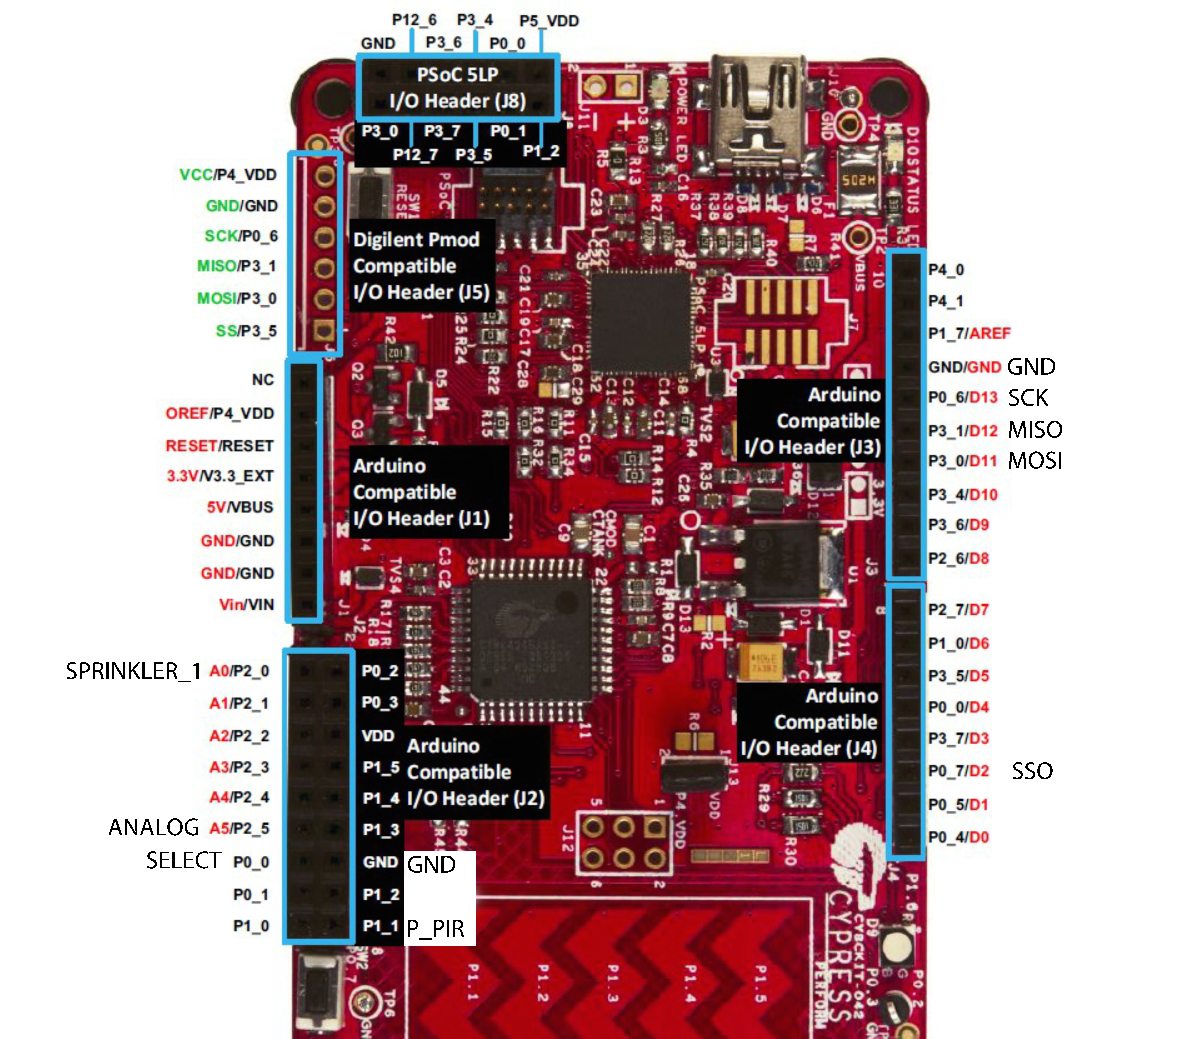
\includegraphics[width=0.7\textwidth]{filer/design/Billeder/psoc4_pin}}
\caption{Oversigt over fysiske pin-navne på PSoC4}
\label{lab:psoc4_pin}
\end{figure}

\newpage
\begin{table}[H]
\subsection{Master (HW)}
Her beskrives hvor mange og hvilke pins der skal benyttes på Devkit8000 til de forskellige forbindelser.
\caption{Tabel der viser pins på Devkit8000}
\begin{small}
\begin{tabular}{|p{3,5cm}|p{2cm}|p{2,9cm}|p{1,6cm}|p{2.6cm}|}
\hline

\textbf{Forbindelse}	&\textbf{Antal pins} 	&\textbf{Signalnavne} &\textbf{Pinnavne} &\textbf{Kommentar}  \\ \hline

SPI 	(P\_DK)			&5 						&MOSI				&J9.1		&					\\\cline{3-4}
					&						&MISO				&J9.2		&					\\\cline{3-4}
					&						&SCK					&J9.5		&					\\\cline{3-4}
					&						&SS0					&J9.3		&					\\\cline{3-4}					
					&						&GND					&J9.20		&					\\\hline

\end{tabular}
\end{small}
\label{table:master_forbindelse}
\end{table}

\begin{figure}[H]
\centering
{\includegraphics[width=\textwidth]{filer/design/Billeder/devkit_j9}}
\caption{Model af tilføjelses-print og J9-stik }
\label{lab:devkit_j9}
\end{figure}


%SW
\section{Softwaredesign}

%SPI
\subsection{SPI (MK PO)}

Der er taget udgangspunkt i HAL Exercise 7\footnote{Hardware abstraktioner. Exercise 7: LDD with SPI. Øvelse med SPI-kommunikation} da SPI blev udarbejdet. Hele kildekoden for Kernemodulet er blevet genbrugt med kun få rettelser. Dele af driveren er også blevet genbrugt. I designet for SPI, er der lagt op til at der skal kunne sendes en 8 bit \verb+CHAR+ ved hver datatransmission. Derfor har det været nødvendigt at rette driveren til, så den kunne håndtere dette.

\subsubsection*{API}

SPI APIen er en klasse med metoder, skrevet ud fra klassebeskrivelserne i software designet, se Projektdokumentation afsnit 6.2.3 Klassebeskrivelser. Implementeringen kan findes på bilags-CD, se CD/SW/Master/Kildekode/spi\_api.

\subsubsection*{Handler}

Handleren er en switchcase i en interrupt-rutine skrevet simultant med APIen, til at handle på forskellige kommandoer sendt fra Master via APIen. Den tilgår interrupt-rutinen ved en SPI transmission og handler i switchcasen udfra hvilken \verb+CHAR+ der modtages. Implementeringen kan findes på bilags-CD, se CD/SW/Enhed/Kildekode/spi\_handler.

% Implementering - sections af HW og SW

\chapter{Implementering}

%HW
\section{Hardwareimplementering}
 


\subsection{PIR-sensor (SK MK)}

PIR-sensoren er en færdigbygget komponent, implementeringen af den er fortaget ved at lave et PIR-API. APIet er lavet i PSoC Creator, den forbinder PIR-sensoren med softwaren. Hvis der registreres bevægelse sættes en input pin på PSoC4 høj og der bliver startet en ISR der kalder en funktion i kontrolleren, som stopper vandingen på banen i 30 min. Yderlig information om PIR-API kan findes i projektdokumentation afsnit 7.7, PIR-API. 

\subsection{Tilslutningsprint (SK)}

Implementeringen af tilslutningsprintet er fortaget ved at konstruere et veroboard print. På figur \ref{fig:Tilslutningsprint_im} kan det færdige resultat ses, samt hvilke tilslutningsmuligheder der er. I projektdokumentationen afsnit 7,2, Tilslutningsprint, kan der findes yderlig information.  

\figur{1}{Tilslutningsprint_implementering}{Tilslutningsprint}{fig:Tilslutningsprint_im}



% Sprinkler pumpe system

\subsection{Sprinkler-pumpe system ()}

Sprinkleren skal forsynes med et vandtryk fra en vandpumpe. Grundfos har doneret en Alpha2 pumpe til formålet. Alpha2 pumpen kræver 230 VAC. Det overskrider hvad der dagligt må arbejde med for studerende på AU. Der er derfor efter aftale med Torben Lund Jensen fra værkstedet givet særskilt tilladelse til at designe og implementere et lukket 230 V / 5 V relæ. Figur \ref{lab:Relay_box} viser kredsløbet for det lukkede 230 V / 5 V relæ. Jordforbindelsen løber direkte igennem og er altid forbundet, mens fasen og nul forbindes/afbrydes af relæet.  

\begin{figure}[H]
  \centering
    \includegraphics[width=0.75\textwidth]{Billeder/230VAC_KREDS}
    \caption{Kredsløbsdiagram for lukket 230 V / 5 V relæ}
    \label{lab:Relay_box}
\end{figure}

\subsubsection{Relæ styring}

PSoC4 giver ikke nok spænding eller strøm til sprinkler relæet, det har derfor været nødvendigt at føre signalet igennem en transistor som det ses på figur \ref{lab:BC517}. Relæet kræver en strøm på 100 mA og den trækker indenfor 3,7 V -8,8 V, dette problem løser BC517 transistoren. 

\begin{figure}[H] \centering
{\includegraphics[width=0.3\textwidth]{Billeder/BC517}}
\caption{BC517 opsætning}
\label{lab:BC517}
\raggedright
\end{figure} 

Modstanden R1 er indsat for at begrænse den strøm der går ind i transistorens base ben, ifølge databladet må base benet højst belastet med 100 mA. Ibase strømmen er beregnet ud fra Ohms lov og der er valgt en modstand på 18 kohm, der begrænser strømmen til 0,1 mA, se formel \ref{eq:Ibase}.

\begin{equation} 
Ibase = \frac{3,3V - 1,4V}{18k\Omega} = 0,1mA
\label{eq:Ibase}
\end{equation} 

Når PSoC4’s pin til BC517 transistoren går høj (3,3V), så skabes der forbindelse mellem collector og emitter på transistoren, herved er der spænding over relæets spole og relæets kontaktsæt klikker herved. Yderlige overvejelser og information kan findes i projektdokumentation afsnit 5.4.3, Relæ-styring.






<<<<<<< HEAD
%% psoc_api

API til styring af PSoC, herunder sensor og sprinkler, er implementeret i PSoC Creator. Top designet består af en ADC\_ SAR\_ Seq og to digitale pins til at styre henholdsvis sprinkler og Select til bestemmelse af temperatur- eller fugtighedsdata for SHT21P.
I top designet er der angivet følgende pins. ''ADC\_ in'', ''SLC'', ''sprinkler'' disse forbindes til henholdsvis pin P2[5], P0[0] og P2[0]. 

Under konfiguration for ADC-komponenten vælges Vref til VDDA og Single ended negative input vælges til Vss. Dette sætter ADCen op til at bruge 0 V som reference spænding.

Da PSoC kun har en SAR komponent er det nødvendigt at initialisere denne i sensorPackage-driveren.

\begin{figure}[htb]
\centering
{\includegraphics[width=0.60\textwidth]{filer/pics/psoc_api_topdesign.png}}
\caption{Top Design for PSoC API}
\label{lab:sht_filter}
\end{figure}

\begin{figure}[htb]
\centering
{\includegraphics[width=0.60\textwidth]{filer/pics/psoc_api_config1.png}}
\caption{Konfiguration af Vref og Single ended negative input}
\label{lab:sht_filter}
\end{figure}

\begin{figure}[htb]
\centering
{\includegraphics[width=0.60\textwidth]{filer/pics/psoc_api_config2.png}}
\caption{Konfiguration af Channels for PSoC API}
\label{lab:sht_filter}
\end{figure}
=======
\subsection{FT-sensor og sprinkler API}

For at hardwaren kan kommunikere korrekt med den høj intellektuelle software, er der oprettet hardware APIer, som sørger for at behandle hardwaren og trække det nødvendige data ud. Dette gør det nemmere, i tilfælde af at en hardwarekomponent med anden virkemåde skal udskiftes, så skal APIen kun rettes til, mens resten af software kan forblive uforandret. 

SHT21p, som er den sensor EasyWater8000 gør brug af, er en analog sensor. Skulle man vælge at skifte sensoren ud til en digital sensor, kræver dette kun en ændring i APIen for at hele systemet virker korrekt igen. 

Disse APIer er udviklet i PSoC Crator med tilhørende PSoC4. 
>>>>>>> FETCH_HEAD


%SW
\section{Softwareimplementering}

%SPI
% SPI IMPLEMENTERING (MIPO)

\subsection{SPI}


% Resultater

\chapter{Resultater}

\section{Software}

På software-siden af projektet er der opnået et responsivt og funktionelt GUI som styres via touch-skærmen på Devkit8000.  Derudover er der opnået at få opsat SPI kommunikation imellem Devkit8000 og PSoC4. På PSoC4-siden er der opnået at få udlæst data fra sensorene og få formateret dem så de er klar til at blive sendt over SPI. Over SPI kommunikationen lykkedes det at sende kommandoer og at hente data fra sensorene så det kan fremvises for brugeren i GUIen.

% Resultater

\chapter{Erfaringer}
\section{Hardwareerfaringer}

Hardwaregruppe har opnået erfaringer indenfor arbejde med SPI, PSoC Creator og kendskab til diverse sensorer. En vigtig erfaring angående SPI er at afstanden imellem Master og Enhed ikke må være for lang, det medførte at signalet blev meget fejlfyldt. Kablet blev kortet ned til ca. 7 cm, som medførte at fejlraten blev minimeret til under 1\%.

I forbindelse med FT-sensoren, erfares det, at det er nemmere at lave API til en analog sensor end til en digital sensor. Signalet fra en analog sensor kan tages direkte, hvor signalet fra en digital sensor kræver ekstra kodning. I vores tilfælde skulle der laves en analog spænding fra en PWM-spænding, som gav yderligere erfaringer inden for opbygning af filtre. 

Da tilslutningsprintet skulle udvikles, var det meget vigtigt at tage hensyn til effektforbruget som skaber varme i spændingsregulatoren. Hvis der ikke blev foretaget korrekt køling kunne komponenten blive beskadiget.  


\section{SW erfaringer}

I software-gruppen har vi for første gang stiftet bekendskab med at skabe en GUI. Denne er lavet i Qt frameworket som det også er første gang vi arbejder i. Vi har også for første gang haft en integreret Git i vores udviklingsværktøj (Qt creator i det her tilfælde) hvilket viste sig at rigtig brugbart. Generelt har arbejdet med Qt og Qt Creator været en fornøjelse da Qt's dokumentation er så veludført. Vi har fået en bedre forståelse for hvordan signaler og events fungerer i et event-dreven system.

I modsætningen til forrige år har vi også haft flere mennesker inde over programmeringen. Hardwarefolk har fået lov til at lave deres drivere til deres hardware. Software-gruppen har lavet dokumentationen så hardwarefolkene vidste hvad de skulle lave. Det har virket rigtig godt og beviser bare at hvis dokumentationen er i orden så kan arbejdet uddeligeres til andre som ikke har været med til at udtænke arkitekturen.

\section{Generelle erfaringer}

Det kan erfares at det er meget vigtigt med korte statusmøder, for at holde hinanden opdateret. I midten af projektet, kørte de forskellige grupper meget individuelt på og det medførte at grupperne mistede overblikket over hvor langt de andre hold var med deres opgaver. En mere specifik gruppekontrakt er at foretrække, da der opstod en del tvivl om hvad konsekvensen var da Jeppe meldte sig ud af gruppen. I forbindelse med at gruppen mistede et medlem, har det været godt at gruppen kunne tilpasse de forskellige arbejdsopgaver efter behov, det indebar at hardware-grupperne kom til at lave en del software. 

Det har været godt med tidlige deadlines, der har presset grupperne til at få lavet de forskellige ting færdig.

Da hele dokumentationen skulle laves færdig  kunne det konstateres at alle billeder skulle gemmes i PDF formatet, i stedet for i PNG format, det gav bedre billedkvalitet og \LaTeX\ reagerede hurtigere.










% Opnåede erfaringer som gruppe

\chapter{Fremtidigt arbejde}

Fremtidigt arbejde for prototypen kunne være at udarbejde et mere kompakt design. Afstanden imellem Master og Enhed skal udvides så Enheden kan være placeret ved hvert golfhul, og Masteren er placeret i en af golfbanens bygninger, hvorfra greenkeeperen kan styre systemet. Denne kommunikation kunne med fordel være trådløs. Ydermere bør der produceres flere Enheder og komponentpakker således at samspillet kan vises for kommende kunder. 

Den midlertidige pumpeløsning bør udskiftes til en fast vandforsyning og sprinklerne skal i stedet styrers af magnetventiler. 

Systemet er pt. ikke sat op til at kunne håndtere flere Enheder. Hvis systemet skal videreudvikles ville dette være et vigtigt punkt. Derudover mangler fejlhåndtering og filstruktur på Masteren. Det er tiltænkt at Enhederne samt loggen skal gemmes i filer, således at data ikke mistes hvis Masteren slukkes.

En yderligere udvidelse af systemet kunne være en app, så greenkeeperen kan styre systemet fra en ekstern enhed. Sprogvalg på Masteren kunne med fordel være en funktion, således at produktet bliver attraktivt på det globale marked, og kan sælges i større omfang.

% Konklusion

\chapter{Konklusion}

Projektets formål har været at udvikle et automatiseret vandingssystem til golfbaner kaldet EasyWater8000. Dette vandingssystem skal vha. sensorer vande når der er brug for det og blokere vandingen når der er folk på de enkelte golfhuller. 

Der er opnået en prototype, som fungerer efter hensigten. Enheden fungerer autonomt og starter vandingen når det er nødvendigt. Aktiveres bevægelsessensoren blokeres vandingen. Gruppen er meget tilfreds med at have en funktionsdygtig  prototype, der opfylder de grundlæggende krav til projektet.  

Gruppen har arbejdet seriøst og fremadrettet med projektet. I forbindelse med brug af ASE-modellen har gruppen været delt op i den fagspecifikke fase. Det har givet muligheden for at de enkelte grupper kunne fordybe sig i bestemte områder, og herved bidrage til det samlede produkt.

Gruppemøderne inklusiv de afholdte trivselsrunder har sørget for at vi som gruppe har haft det godt med hinanden og eventuelle problemer kunne afklares i tide. Optil udmeldelsen af Jeppe Stærk var der en del frustration omkring hvorvidt han havde tænkt sig at genoptage projektarbejdet og skolen generelt. Efter udmeldelsen af Jeppe Stærk kunne gruppen igen arbejde koncentreret og fremadrettet, det betød også at hele opgavefordelingen blev genfordelt.  

Det kan konkluderes af udviklingsværktøjet \LaTeX \ er rigtig smart ved store gruppeopgaver, da man sparer meget tid på opsætningen af rapporten og layout.








% Individuel Konklusion

\include{filer/Individuelkonklusion}

% Individuel Konklusion

% Litteraturliste
\chapter{Litteraturliste}
Foruden de tilgængelige Campus-dokumenter i forbindelse med EPRJ3 er nedenstående litteratur benyttet. 

\section{Bøger}
Analogteknik T-005, Tore Skogberg, 2014

T-133 UML-Light, Finn Overgaard Hansen, 2013, Ingeniørhøjskolen Aarhus Universitet

\section{Hjemmesider}

\url{http://qt-project.org}, Qt Project Hosting [2014-12-10]


\section{Opslagsværker}



% Billags-CD struktur
\chapter{Bilags-CD indhold}

Figur \ref{fig:Bilags_CD} viser oversigten over filstrukturen på den vedlagt CD med bilag.

\begin{figure}[H]
  \centering
    \includegraphics[height=0.7\textheight]{billeder/bilagscd}
    \caption{Filstruktur for bilags-CD}
    \label{fig:Bilags_CD}
\end{figure}

\end{document}
